\documentclass[a4paper,oneside]{mystyle}

% custom packages
\usepackage{empheq}
\usepackage{graphicx}
\usepackage[font={small}]{caption}
\usepackage{subcaption}
\usepackage{framed}
\usepackage{listings}
\usepackage{wrapfig}
\usepackage{sidecap}
\usepackage{xcolor}
\usepackage{lineno}
\usepackage{marvosym}
\usepackage{xstring}
\usepackage{mfirstuc}
\usepackage{pdfpages}
\usepackage{lipsum}
\usepackage{lettrine}
\usepackage[explicit]{titlesec}
\usepackage{cancel}
\usepackage[noabbrev]{cleveref}
\usepackage{indentfirst}
\usepackage{mathtools}
\usepackage{algorithmicx}
\usepackage{algpseudocode}
\usepackage{algorithm}
\usepackage{hyperref}
\usepackage{nicefrac}
\usepackage{booktabs}
\usepackage{amsmath}

%%%%%%%%%%%%%%%%%%%%%%%%%%%%%%%%%%%%%%%%%%%%%%%%%%%%%%%%%%%%%%%%%%%%%
% DOCUMENT METADATA

\thesistype{Master thesis}
\title{Evaluating perception in industrial scenarios: tools, metrics and benchmarks}

\author{Daniele Evangelista}
\email{evangelista.1665872@studenti.uniroma1.it}
\institute{RoCoCo - Cognitive robot teams laboratory\\[2pt]
Department of Computer, Control and Management Engineering Antonio Ruberti\\[2pt]
Sapienza University of Rome}

\supervisors{Eng.\ Dr.\ Alberto Pretto}
%\cosupervisors{Eng.\ Dominik Schlegel}

\date{\today}

%%%%%%%%%%%%%%%%%%%%%%%%%%%%%%%%%%%%%%%%%%%%%%%%%%%%
\lstset { %
	language=C++,
	backgroundcolor=\color{black!5}, % set backgroundcolor
	basicstyle=\footnotesize,% basic font setting
}

%ds colors
\definecolor{orange}{rgb}{1,0.4,0}
\definecolor{green}{rgb}{0,0.5,0}

%ds referencing
\newcommand{\myref}[3]{\hyperref[#1]{#2} (\capitalisewords{#3} \ref{#1})}

%ds blue box
\definecolor{myblue}{rgb}{.9, .9, 1}

\newlength\mytemplen
\newsavebox\mytempbox
\newcommand*\widefbox[1]{\fbox{\hspace{2em}#1\hspace{2em}}}

\makeatletter
\newcommand\mybluebox{%
	\@ifnextchar[%]
	{\@mybluebox}%
	{\@mybluebox[0pt]}}

\def\@mybluebox[#1]{%
	\@ifnextchar[%]
	{\@@mybluebox[#1]}%
	{\@@mybluebox[#1][0pt]}}

\def\@@mybluebox[#1][#2]#3{
	\sbox\mytempbox{#3}%
	\mytemplen\ht\mytempbox
	\advance\mytemplen #1\relax
	\ht\mytempbox\mytemplen
	\mytemplen\dp\mytempbox
	\advance\mytemplen #2\relax
	\dp\mytempbox\mytemplen
	\colorbox{myblue}{\hspace{1em}\usebox{\mytempbox}\hspace{1em}}}

%ds global definitions
\def\g2o{\texttt{g2o}}
\def\zero{\mathbf{0}}
\def\P{\mathcal P}
\def\p{\mathbf{p}}
\def\tp{\tilde{\p}}
\def\tab{\phantom{tab}}
\def\homx{\mathbf{\tilde{x}}}
\def\trans{\mathbf{t}}
\def\quat{\mathbf{q}}
\def\state{\mathbf{x}}
\def\SState{\mathbf{X}}
\def\meas{\mathbf{z}}
\def\tmeas{\tilde{\meas}}
\def\Meas{\mathbf{Z}}
\def\pred{\hat{\meas}}
\def\Pred{\hat{\Meas}}
\def\linstate{\breve{\state}}
\def\Linstate{\breve{\SState}}
\def\optstate{\state^\star}
\def\Optstate{\State^\star}
\def\dx{\Delta \state}
\def\dz{\Delta \meas}
\def\hessian{\mathbf{H}}
\def\bvec{\mathbf{b}}
\def\error{\mathbf{e}}
\def\terror{\tilde{\error}}
\def\jacob{\mathbf{J}}
\def\tjacob{\tilde{\jacob}}
\def\l{\mathbf{l}}
\def\L{\mathbf{L}}
\def\u{\mathbf{u}}
\def\U{\mathbf{U}}
\def\k{\mathbf{k}}
\def\S{\mathbf{S}}
\def\kdtree{\textit{K}-D tree}
\def\T#1#2{^{#1}T_{#2}}
\def\rot{\mathbf{R}}
\def\v2t{\text{v2t}}
\def\flatten#1{\text{flatten}\left({#1}\right)}
\def\t2v#1#2{^{#1}\tau_{#2}}
\def\deltat2v#1#2{^{#1}\Delta\tau_{#2}}
\def\norm#1{\|{#1}\|}
\def\skew#1{{\lfloor{#1}\rfloor}_\times}
\def\chref#1{Chapter~\ref{ch:#1}}
\def\secref#1{Sec.~\ref{#1}}
\def\figref#1{Fig.~\ref{#1}}
\def\tabref#1{Tab.~\ref{#1}}
\def\eqref#1{Eq.~(\ref{#1})}
\def\algref#1{Alg.~\ref{#1}}
\def\lstref#1{Lst.~\ref{#1}}
\def\ourmethod{\textit{g2o\_slim~}}
\renewcommand{\thesubfigure}{\Alph{subfigure}}

% mathemagical stuff
\DeclareMathOperator*{\argmax}{argmax}
\DeclareMathOperator*{\argmin}{argmin}
\newcommand{\pluseq}{\mathrel{+}=}
\newcommand{\asteq}{\mathrel{*}=}

% indentation stuff
\newlength\myindent
\setlength\myindent{2em}
\newcommand\bindent{%
    \begingroup
    \setlength{\itemindent}{\myindent}
    \addtolength{\algorithmicindent}{\myindent}
}
\newcommand\eindent{\endgroup}

\newcommand\mynote[1]{\textcolor{red}{#1}}

\begin{document}
	
\frontmatter
\begin{titlepage}
\maketitle
\cleardoublepage\null
\thispagestyle{empty}
\end{titlepage}

\newcounter{notation}
\begin{abstract}
To do ... 
\end{abstract}

\chapter*{Nomenclature}\label{ch:symbols}
\addcontentsline{toc}{chapter}{Nomenclature}

%\section*{Notation}
%\refstepcounter{notation}
%\label{sec:notation}
%
%To do ...
%\begin{tabbing}
%	\hspace*{3.0cm}		\= \kill
%	$^A\rot_{B}(\alpha, \beta, \gamma)$ \> Rotation from frame A to frame B expressed in A \\[0.75ex]
%	$^A\trans_{B}(t_x,t_y,t_z)$ \> Translation from frame A to frame B expressed in A  \\[0.75ex]
%	$\T{A}{B}(R,\trans)$ \> Transformation from frame A to B expressed in A  \\[0.75ex]
%	$\t2v{A}{B}(R,\trans)$ \> Transformation from frame A to B expressed in A (vectorized) \\[0.75ex]
%	${\lfloor\trans\rfloor}_\times$ \> Skew-symmetric matrix of a vector $\mathbf{t} \in \mathbb{R}^{3\times3}$
%\end{tabbing}

\section*{Acronyms and Abbreviations}
\label{sec:acronyms}

\begin{tabbing}
	\hspace*{3.5cm}		\= \kill
	API \> Application Programming Interface \\[1ex]
	GUI \> Graphical User Interface \\[1ex]
	CNN \> Convolutional Neural Network \\[1ex]
	MLP \> Multi-Layer Perceptron \\[1ex]
	OpenCV  \> Open source Computer Vision (library), \url{www.opencv.org} \\[1ex]
	Git  \> Git revision control, \url{www.git-scm.com} \\[1ex]
	RBP  \> Random Bin Picking \\[1ex]
	PPT  \> Pick and Place Task \\[1ex]
	IoU  \> Intersection over Union \\[1ex]
	AD  \> Average Distance \\[1ex]
	VSD  \> Visible Surface Distance \\[1ex]
	d.o.f.  \> Degrees of freedom \\[1ex]	
\end{tabbing}

\clearpage

\tableofcontents
\listoffigures
\listoftables
\mainmatter
\newpage
\chapter{Introduction}\label{ch:intro}
To do ...
\newpage
\chapter{Perception and Sensing in Robotics: Sensors and Algorithms}\label{ch:perceptionandsensing}
In this chapter we will talk about perception in industrial settings, focusing the attention on the tools, e.g. sensors and software, and the techniques used to solve industrial problems such as Random Bin Picking (RBP) and Pick\&Place (PPT) of objects. In the end we will focus also on the state of the art software libraries that nowadays are commonly used and tested in the industrial settings.

\section{Robotics in Industry}\label{sec:roboticsinindustry}
Over the years, industry has been one of the most active sector where robots and automated systems spread and diffused without limits. This is basically due to the fact that robots can easily complete tasks that humans are not capable at all, both for physical and technical failings. Robots are capable of compute the same operation multiple times without loosing any kind of accuracy and precision, they are repetitive, fast, and very well suited for industrial application, where most of the time being fast and accurate are two central points of the productive chain.

Manufacturing is one of the industrial sectors that saw the robotics ``era'' growing faster than elsewhere. Into the factories, robots are involved in every ring of the productive chain, from heavy loads handling to precise and accurate placing, from iron and metal soldering to small part assembly. The higher accuracy and velocity that robots can reach, with so high levels of repeatability and precision, brought robots, manipulators particular, at the top level of the industrial necessities.

\begin{figure}
    \centering
    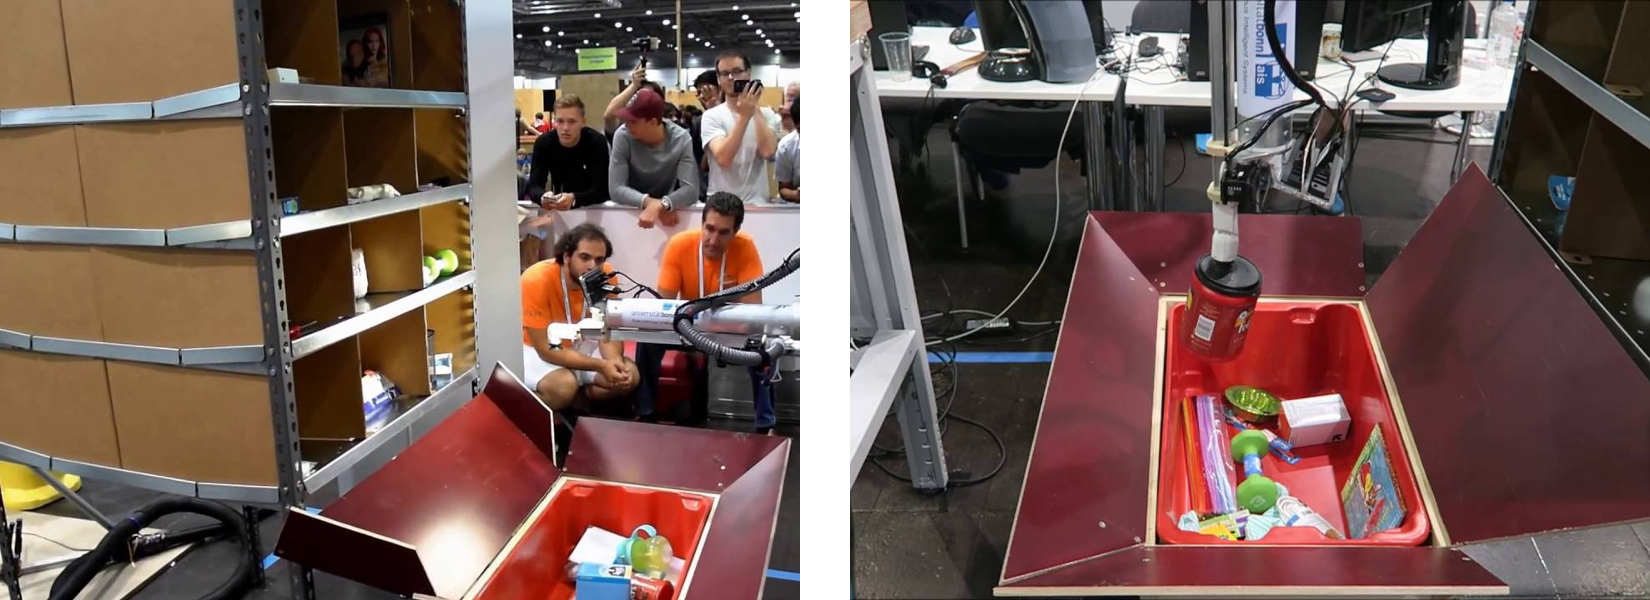
\includegraphics[width=0.8\textwidth]{figures/1_perception_and_sensing_in_robotics/amazon_picking_ch}
    \caption{\textbf{Amazon Picking Challenge example scenario.} In the images, the team is trying to detect and grasp objects from the red bin on the bottom, and place them on the shelf.} 
    \label{fig:amazon_picking_ch}
\end{figure}

The importance of robots in the industrial sector is supported also by big companies, such as Amazon, Google and others, that in the last years demonstrated high interests in investing and developing their technologies in order to improve their performance and business. One particular example of how big companies invest in robotics is the Amazon Picking Challenge competition proposed the first time at the International Conference on Intelligent Robots and Systems (IROS) in 2015 by the Amazon Robotics division\footnote{https://www.amazonrobotics.com}. This competition is thought to enhance and improve the research in the robotic manipulation, focusing the attention in grasping from random and highly cluttered environments, such as warehouse shelves or bins full of irregular and messy objects. In Figure \ref{fig:amazon_picking_ch} there are some examples of what are the typical scenarios where the teams that participate to this kind of events have to compete.

\subsection{Random Bin Picking (RBP)}\label{subsec:binpicking}
To do ...

\subsection{Pick\&Place Tasks (PPT)}\label{subsec:pickandplace}
To do ...

\section{3D Reconstruction}\label{sec:3dreconstruction}
To do ...

\section{Object Detection}\label{sec:objectdetection}
To do ...

\section{State of the art Software Libraries in Industry}\label{sec:industrylibraries}
Machine Vision is one of the most active area in industrial settings. Over the past years, many software companies and Open Source communities have dedicated lot of effort in developing robust and effective techniques and algorithms in order to assist industrial realities, such as companies and start ups, in performing computer vision assisted tasks, e.g. random bin picking, Pick\&Place tasks and so on.

In the following subsection a list of tools and libraries will be introduced, focusing mainly on the MVTec's Halcon Libraries, which are the one that we used in the experiment phase of this work. 

\subsection{Halcon Libraries}\label{subsec:halconlibs}
Halcon\footnote{http://www.mvtec.com/products/halcon/}, from MVTec, is a set of commercial software developed and sold explicitly for industrial settings. Over the past 5 years it has become the state of the art in machine vision for industrial tasks. It serves all industries with an extensive library of more than 1600 operators for blob analysis, morphology, matching, measuring, identification, and 3D vision, to name just a few.

The full library can be accessed from common programming languages like C, C++, C\#, Visual Basic .NET, and Delphi. In particular, our tests have been developed using the C++ APIs. In the following chapters we will test this standard Machine Vision approaches over the RAW and T-Less datasets, and compare them with completely different approaches such as Deep Learning CNNs for object localization and recognition.

\begin{figure}
    \centering
    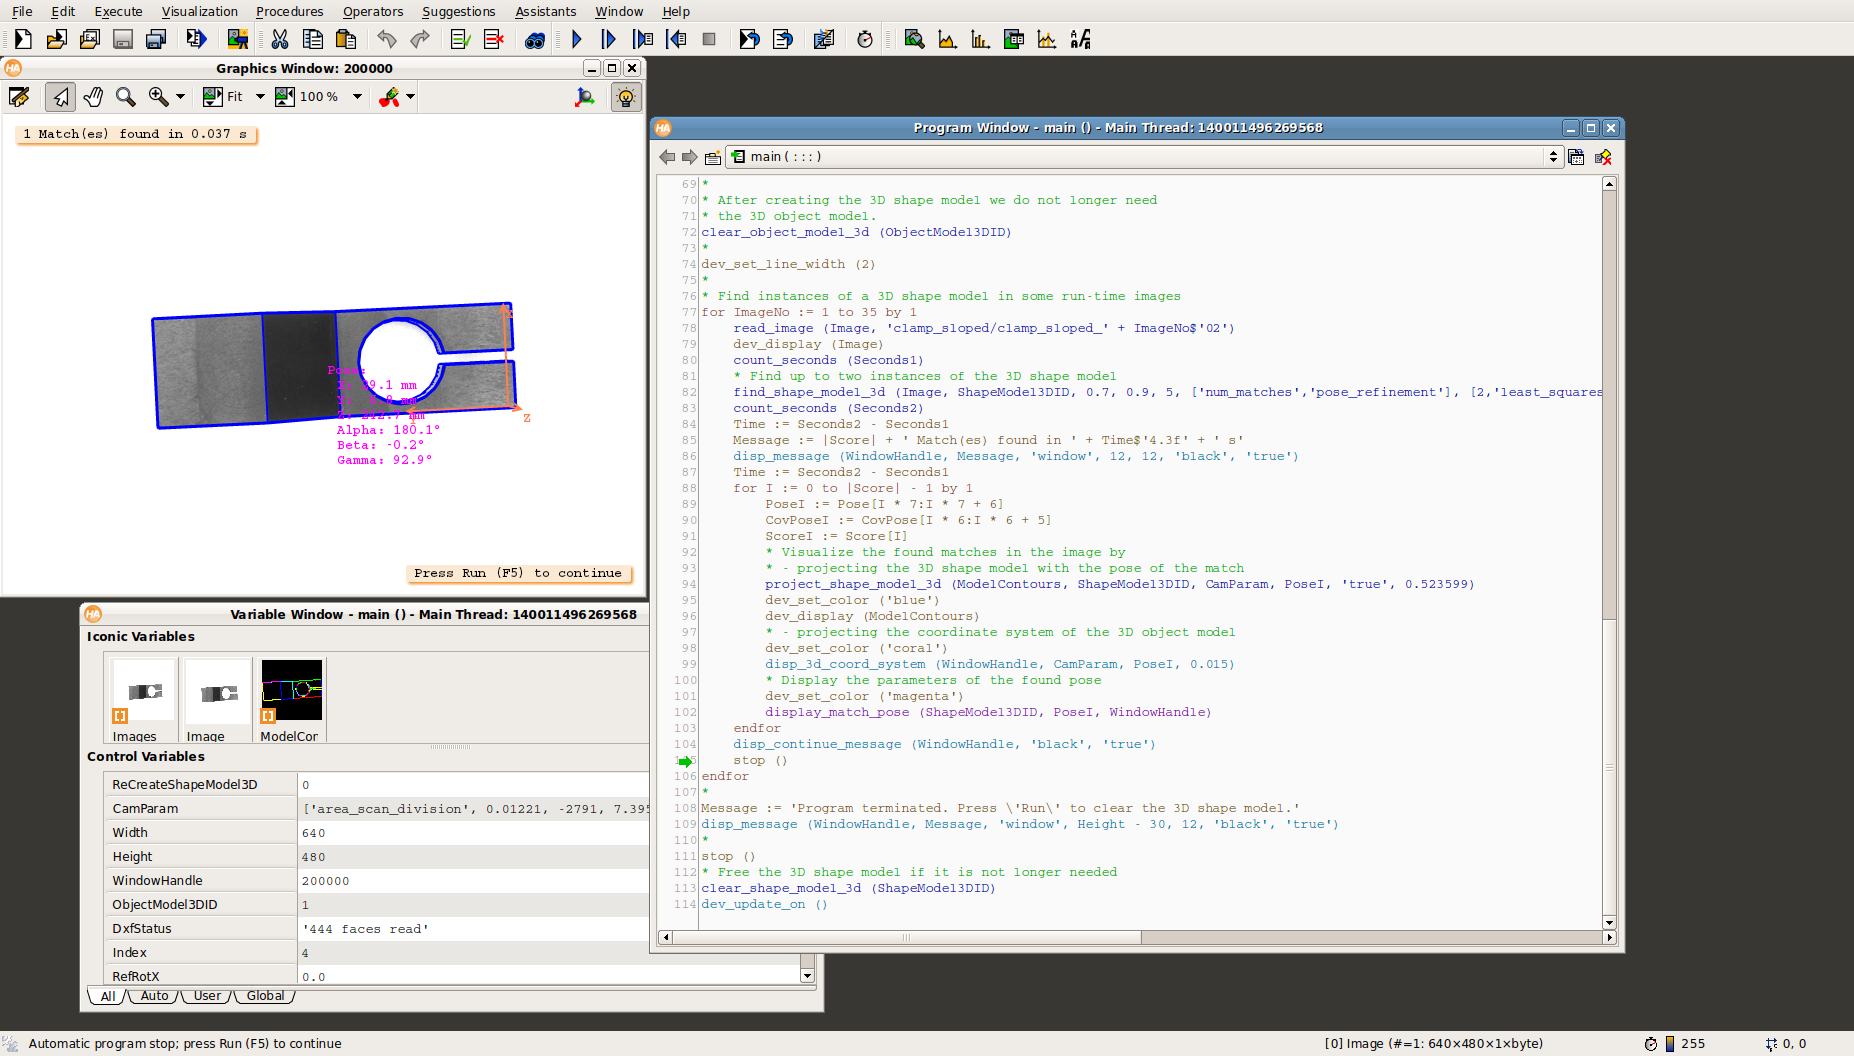
\includegraphics[width=0.8\textwidth]{figures/1_perception_and_sensing_in_robotics/hdevelop_gui_example}
    \caption{\textbf{Hdevelop GUI example.} An example of using the Hdevelop software from the Halcon Libraries. In particular here we are performing an object detection and localization task.} 
    \label{fig:hdevelop_example}
\end{figure}

The Halcon Library has also an interactive and friendly GUI, provided in order to facilitate the interfacing with the low level software APIs. The aforementioned software tool is called HDevelop, and an example of its usage and graphical interface is depicted in Figure \ref{fig:hdevelop_example}.

As anticipated, this software library is under commercial license, and our distribution has been sold to La Sapienza University of Rome that can use it for research and other non-commercial purposes. 

\begin{figure}
    \centering
    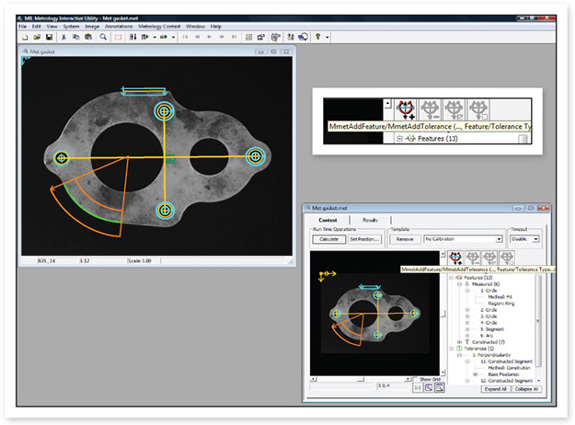
\includegraphics[width=0.8\textwidth]{figures/1_perception_and_sensing_in_robotics/mil_gui_example}
    \caption{\textbf{MIL GUI example.} The graphical user interface of the Matrox Imaging Library.} 
    \label{fig:mil_example}
\end{figure}

\subsection{Matrox Imaging Library (MIL)}\label{subsec:mil}
Another important software library that needs to be mentioned is the Matrox Imaging Library\footnote{https://www.matrox.com/imaging/en/products/software/mil/} (MIL). MIL is a complete collection of software tools for developing machine vision in lots of different scenarios, it is not restricted to the industrial one such as for the previously mentioned Halcon Libraries, but it covers also medical images applications and many others.

MIL includes also a graphic user interface for fast developing and prototyping of solutions. An example of this GUI is depicted in Figure \ref{fig:mil_example}.

This library is not part of the tests and examples performed during this work.
\newpage
\chapter{Benchmarks and Metrics in Industry}\label{ch:benchmarks_and_metrics}
In this chapter all the tools and the benchmarks for object localization and detection will be exposed. In particular, first the metrics and the techniques used to evaluate pose estimations will be presented, then some publicly available datasets will be presented. 

The problems that are going to be tackled are related to the 6D object pose estimation task. A 6D object pose is mathematically the 3D position of the object in the space plus 3 more terms that describe its rotation:

\begin{equation}
    \label{eq:6D_obj_pose_0}
    \hat{P} = (x, y, z, \alpha_x, \alpha_y, \alpha_z)^T
\end{equation}

The Eq. \ref{eq:6D_obj_pose_0} refers to the 6D pose estimate of an object, the first three terms $x, y, z$ describe the position in the camera reference frame, while the last three terms $\alpha_x, \alpha_y, \alpha_z$ represent the object's rotation angles along the $x, y, z$ camera axis respectively. This formulation can be easily manipulated in terms of rotation matrices and translation vectors:

\begin{equation}
    \label{eq:6D_obj_pose_1}
    \hat{P} = (R, t)
\end{equation}

The Eq. \ref{eq:6D_obj_pose_1} is a manipulated version of \ref{eq:6D_obj_pose_0} where the rotation matrix $R$ encodes the three angles of rotation $\alpha_x, \alpha_y, \alpha_z$ and the translation vector $t$ encodes the $x, y, z$ position of the object in the reference frame of the camera.

\begin{figure}
	\centering
	\begin{subfigure}{.5\textwidth}
  		\centering
  		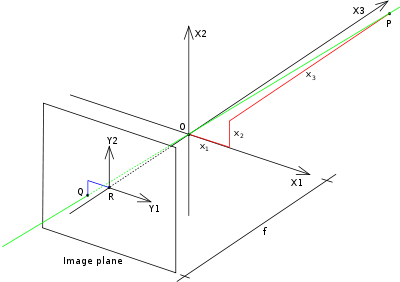
\includegraphics[width=.9\linewidth]{figures/2_benchmarks_and_metrics/pinhole_geometry_3D}
  		\caption{3D view}
  		\label{fig:pinhole_geometry3D}
	\end{subfigure}%
	\begin{subfigure}{.5\textwidth}
  		\centering
  		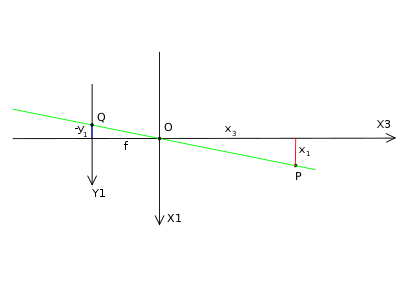
\includegraphics[width=.9\linewidth]{figures/2_benchmarks_and_metrics/pinhole_geometry_2D}
  		\caption{2D view}
  		\label{fig:pinhole_geometry2D}
	\end{subfigure}
	\caption{\textbf{Pinhole Camera Geometry.} In (A) the geometry of the pinhole camera in 3D view, in (B) its 2D representation.}
	\label{fig:pinhole_geometry}
\end{figure}

Each object pose estimate can also be projected back to the camera image plane. This projection between the 3D space and the 2D space of the image plane is achieved by applying the projection obtained with a given camera matrix model. The camera model that we consider here is the so called Pinhole Camera Model, and it's geometry is depicted in Figure \ref{fig:pinhole_geometry}.

The mapping from the coordinates of a 3D point $P$ to the 2D image coordinates of the point's projection onto the image plane, according to the pinhole camera model is given by:

\begin{equation}
    \label{eq:3D_to_2D_mapping}
    x_i = \left[ \begin{array}{c} u \\ v \end{array} \right] = \dfrac{f}{x_3} \left[ \begin{array}{c} x_1 \\ x_2 \end{array} \right]
\end{equation}

In Eq. \ref{eq:3D_to_2D_mapping} $x_1, x_2, x_3$ represent the 3D position in space of a generic point, $f$ is the focal length of the camera, and $u, v$ are the image coordinates obtained after the projection.

The formulation just explained is for an ideal pinhole camera located in the origin and with focal length equal for the $x$ and $y$ axes of the image. Typically, the situation is different, and the more generic formulation is like the following:

\begin{equation}
    \label{eq:generic_pinhole_camera_model}
    x_i = \left[ \begin{array}{c} u \\ v \\ 1 \end{array} \right] = \begin{bmatrix} f_x & 0 & c_x \\ 0 & f_y & c_y \\ 0 & 0 & 1 \end{bmatrix} \left[ \begin{array}{c} x_1 \\ x_2 \\ x_3 \end{array} \right]
\end{equation}

In Eq. \ref{eq:generic_pinhole_camera_model} the camera is formulated using its internal parameter $f_x, f_y, c_x, c_y$ that represent respectively the two focal lengths on the $x, y$ image axis and the camera optical center $(c_x, c_y)^T$.

With Eq. \ref{eq:3D_to_2D_mapping} and \ref{eq:generic_pinhole_camera_model} we can project each point of the 3D object model onto the image plane and compare the estimated pose with the ground truth one following one of the metrics that are going to be explained in the sections below.

\section{Metrics}\label{sec:metrics}
The problem of evaluating how good is a pose estimate w.r.t. the ground truth is a challenging and still very open topic in computer vision community.  Taking inspiration from \cite{hodan20166DPoseEstimation} we will first focus on bounding box estimates comparison and then will pass to the more complex and challenging problem of compare two object 6D pose estimate.

\begin{figure}
    \centering
    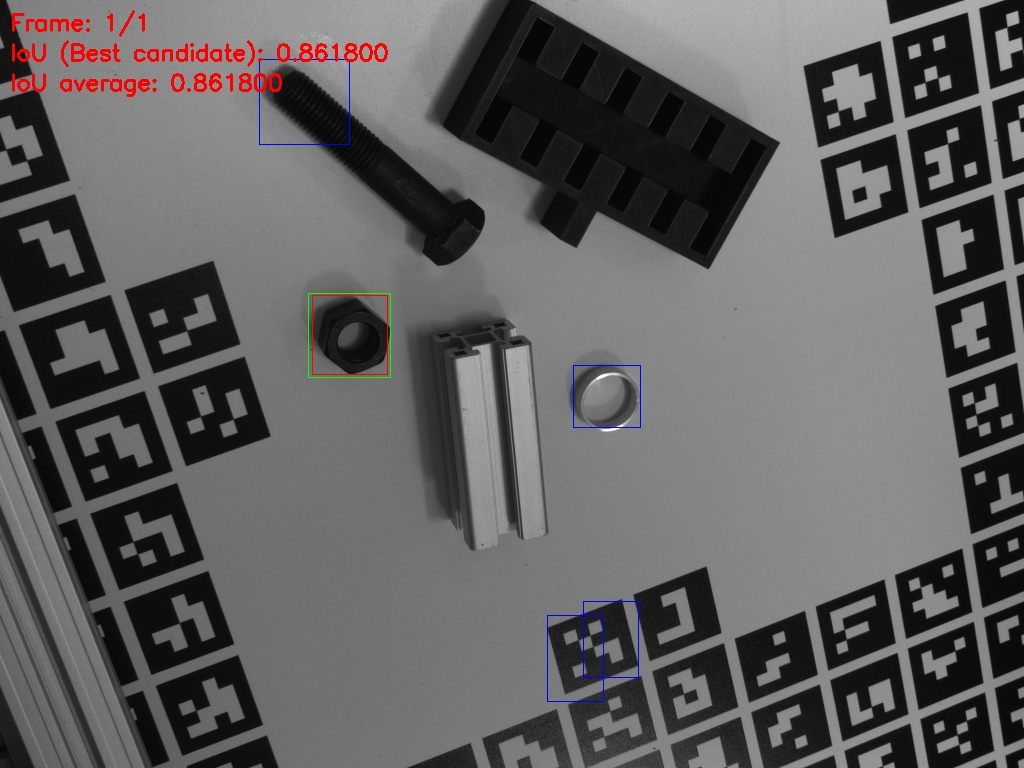
\includegraphics[width=0.7\textwidth]{figures/2_benchmarks_and_metrics/iou_example}
    \caption{\textbf{IoU score estimation example.} An eample of estimating the 2D bounding box of an object, in particular, the small nut, called M20 in the RAW dataset, with the Halcon Libraries. In red the ground truth bouning box, in green the Halcon best candidates, in blue the last two best candidates.} 
    \label{fig:iou_example}
\end{figure}

\subsection{2D Intersection over Union (IoU)}\label{subsec:iou}
The most common way to measure accuracy of object detection in 2D domain is to calculate the Intersection over Union score \cite{everingham2015challenge}:

\begin{equation}
    \label{eq:iou_score}
    s_{IOU}(\hat{B}, \bar{B}) = \dfrac{area(\hat{B} \cap \bar{B})}{area(\hat{B} \cup \bar{B})}
\end{equation}

In Eq. \ref{eq:iou_score} $\hat{B}$ and $\bar{B}$ are the estimated and ground truth 2D region respectively. Depending on the task, $\hat{B}$ and $\bar{B}$ can be rectangular regions (given by bounding boxes) or segmentation masks. For evaluation of 6D object pose estimates, the 2D regions can be obtained by projection of the object model $\mathit{M}$ in the estimated pose $\hat{P}$ and the ground truth pose $\bar{P}$ . Such pose error function is ambiguity-invariant, but since it operates in the projective space, it provides only a weak information about fitness of the object surface alignment. That basically means that every projection of the model that realizes in the same bounding box will have the very same score, even if the object is completely flipped among the two 6D poses. It is said that the IoU score is not ambiguity-invariant, we will see in the further section what ambiguity is. 

That is the reason why we only consider IoU for 2D measurement comparison, and so, only for object detection tasks, where just the location of the object within the image plane is considered to be interesting, not its exact position and orientation in 3D space. Examples of bounding boxes comparison, so IoU estimation is given in Figure \ref{fig:iou_example}. Usually a object detection is considered correct, when the IoU score of 2D bounding boxes of an object in the estimated and the ground truth pose is above a
threshold (e.g. 0.5).

\subsection{5cm, 5deg criteria}\label{subsec:5cm5deg}
After having introduced the metrics used for comparing object detection estimates, we now pass to tackle the problem of estimating the ``goodness'' of a 6D pose estimate. In the introduction of chapter \ref{ch:benchmarks_and_metrics} we formulated the pose of an object in 3D space in terms of rotation  matrix and translation vector, as stated in Eq. \ref{eq:6D_obj_pose_1}. From this simple formulation, intuitively, a simple error function can be built, in particular we can consider the error of the estimated pose $\hat{P} = (\hat{R}, \hat{t})$ w.r.t. the ground truth pose $\bar{P} = (\bar{R}, \bar{t})$ as composed by two independent terms, the translational error $(e_{TE})$ and the rotational error $e_{RE}$ respectively. These errors can be used as a metric for the computation of the goodness of a 6D pose estimate.

More in detail, the aforementioned $e_{TE}$ and $e_{RE}$ can be mathematically expressed as:

\begin{equation}
    \label{eq:translational_error}
    e_{TE}(\hat{t}, \bar{t}) = \norm{\hat{t} - \bar{t}}_2
\end{equation}

\begin{equation}
    \label{eq:rotational_error}
    e_{RE}(\hat{R}, \bar{R}) = arccos(\dfrac{Tr(\hat{R}\bar{R}^{-1}) - 1}{2})
\end{equation}

In particular, Eq. \ref{eq:translational_error} is simply the squared distance from the 2 points represented by their respective translation vectors $\hat{t}$ and $\bar{t}$, and Eq. \ref{eq:rotational_error} represents the rotational error in the axis-angle representation of the rotation matrices $\hat{R}$ and $\bar{R}$. More over, in $e_{RE}$, the function $Tr()$ is the trace of the rotation matrix.

After the previous formulation, we can now introduce a simple and intuitive criteria for evaluating the goodness of a 6D pose estimate. In \cite{shotton2013coordinate}, the so called \emph{5cm, 5deg} criteria have been introduced. It simply states that it is considered a good pose estimate if and only if $e_{TE} \leq 5cm$ and $e_{RE} \leq 5deg$. Of course, more general formulation of the same criteria can be used, by imposing variable thresholds $t_{TE}$ and $t_{RE}$ in the place of the constants $5cm$ and $5deg$.

This criteria was initially used for evaluating camera pose estimations, and it perfectly fits the case, but in terms of computing the goodness of a 6D object pose estimate, it is not adaptive to object model projections, in the sense that 2 different poses that refer to 2 different model projection onto the image plane can assume the very same $e_{TE}$ and $e_{RE}$, so those errors are still not ambiguity-invariant, as like as the IoU score.

\subsection{Pose Ambiguity Invariant Metrics}\label{subsec:pose_ambig_invariant_metrics}
Before introducing the idea of Average Distance for model points let's introduce the concept of \emph{Indistinguishable Poses} and \emph{Invariance to Pose Ambiguity}. As anticipated in the last two sections, IoU score and rotational and translational errors are not invariant to pose ambiguities, so let's see what this concern before introducing how we can overcome this issue.

\subsubsection{Indistinguishable Poses}\label{subsubsec:indistinguishable_poses}
If we take as example a generic object model, call it $M$, we can define a class of \emph{indistinguishable} poses for this model with the following:

\begin{equation}
    \label{eq:indistinguishable_poses}
    [P]_{M,I,\epsilon} = {P^{\prime} : d(v_I[PM], v_I[P^{\prime}M]) \leq \epsilon}
\end{equation}

where $v_I[M] \subseteq M$ is that part of the object model M that is actually visible in the image $I$, that is not self-occluded or occluded by some other object, $d$ is a distance between the surfaces, and $\epsilon$ is a threshold that basically controls the level of detail that we want to achieve in comparing two different views of the same model in the image.

\subsubsection{Invariance to Pose Ambiguity}\label{subsubsec:pose_ambiguity_invariance}
Pose Ambiguity is a necessary property for a 6D object pose estimator. Given an image $I$, a model $M$ and an estimated pose $\hat{P}$, the error $e(\hat{P}, \bar{P}; M, I)$ is required to be invariant under pose ambiguity iff:

\begin{equation}
    \label{eq:pose_ambiguity_invariance}
    \forall \hat{P}^\prime \in [\hat{P}]_{M, I, \epsilon},
    \forall \bar{P}^\prime \in [\bar{P}]_{M, I, \epsilon} : 
    e(\hat{P}^\prime, \bar{P}^\prime) \approx e(\hat{P}, \bar{P})
\end{equation}

where the approximation is given because of the $\epsilon$ tolerance term. A pose error function $e$ that satisfy such property is called \emph{ambiguity-invariant}.

This property is extremely important because an 6D object pose estimator relies its estimates only on the single image, there is no tracking information, and any other spatial relation with the model pose in the image that can distinguish two different pose estimates, so pose ambiguity cannot be removed in any way, that is why we need to model it somehow.

\subsubsection{Average Distance (AD)}\label{subsubsec:average_distance}
When the sets of visible points for the model $M$ in the image $I$ is available, one possible solution to estimate how good is the detected pose $\hat{P}$ is to evaluate the average of the maximum of distances between corresponding points of model $M$ for each pose pair $(\hat{P}, \bar{P}) \in Q = [\hat{P}]_{M, I, \epsilon} \times [\bar{P}]_{M, I, \epsilon}$, and finally take the minimum of those average distances:

\begin{equation}
    \label{eq:average_distance}
    d_h((\hat{R}, \hat{t}), (\bar{R}, \bar{t}); M) = \dfrac{1}{|M|}  \sum\nolimits_{x_1 \in M} \min_{x_2 \in M} \norm{(\hat{R}x_1 + \hat{t}) - (\bar{R}x_2 + \bar{t})}_2
\end{equation}

This distance is very intuitive, but not so effective, and we will see whit an example in the following subsection why take the maximum instead of the average, is a more convenient way.

\begin{figure}
    \centering
    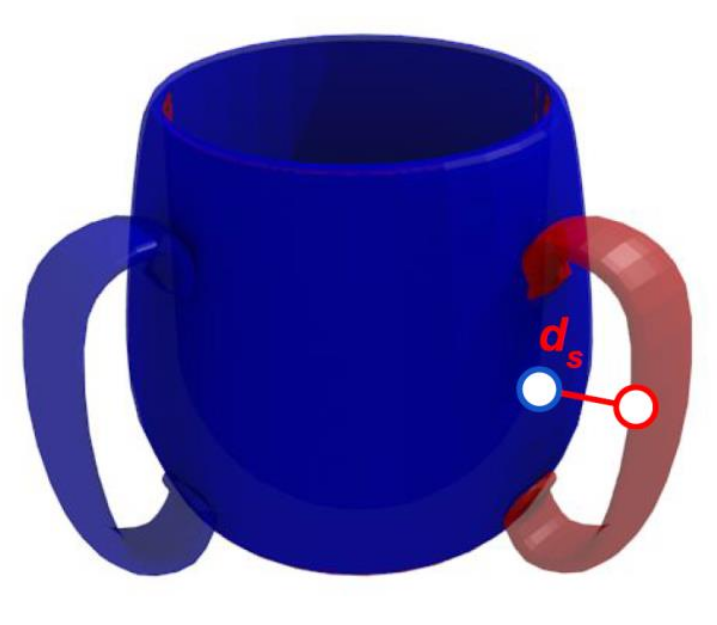
\includegraphics[width=0.5\textwidth]{figures/2_benchmarks_and_metrics/max_av_distances_example}
    \caption{\textbf{Maximum vs Average Distance.} In this example, it is perfectly shown how taking the maximum instead of the average, is much more convenient. For the mug depicted in the picture, the blue pose (the ground truth), and the red one (the estimation) have very low average distance, while high maximum distance. This explain how maximum distance is more convenient for this case, it reflects better the misalignment between the two poses. The average distance $d_h$ cannot be drawn here, because this distance does not relates with any geometrical points, it's just a score.} 
    \label{fig:max_av_distances_example}
\end{figure}

\subsubsection{Maximum Distance (MD)}\label{subsubsec:average_distance}
As anticipated in the last section, taking the maximum instead of the average, can be more effective, also compared with the task that we want to perform. Imagine to take a mug, like in the example in Figure \ref{fig:max_av_distances_example}, where the Maximum Distance $d_s$ is calculated performing the maximum instead of the average:

\begin{equation}
    \label{eq:maximum_distance}
    d_s((\hat{R}, \hat{t}), (\bar{R}, \bar{t}); M) = \max_{x_1 \in M} \min_{x_2 \in M} \norm{(\hat{R}x_1 + \hat{t}) - (\bar{R}x_2 + \bar{t})}_2
\end{equation}

Whit this little modification to the formulation of the distances, the situation completely changes. In the example in Figure \ref{fig:max_av_distances_example} the distance $d_s$ reflects better the misalignment between the estimated pose and the ground truth. But, is this the right choice? Is this distance reflecting all the necessary when estimating the pose of the mug? In Figure \ref{fig:ds_vs_dp} there is another possible distance that can reflect better the misalignment between ground truth and estimated pose. It is clearly evident that maybe the new distance $d_p$, is better that the maximum distance $d_s$. So we need to find a solution to this problem, and one possible way is to introduce the concept of \emph{equivalence classes}, and then calculate the distances also considering them.

Considers all poses from the equivalence class $[(\hat{R}, \hat{t})]$ of the ground truth pose (given by pre-defined symmetries of the object), we can define the new distance $d_p$ with the following:

\begin{equation}
    \label{eq:maximum_distance_eq_classes}
    d_p((\hat{R}, \hat{t}), (\bar{R}, \bar{t}); M) = \min_{(\hat{R}, \hat{t}) \in [(\hat{R}, \hat{t})]} \max_{x \in M} \norm{(\hat{R}x + \hat{t}) - (\bar{R}x + \bar{t})}_2
\end{equation}

This new distance reflects better the misalignment between ground truth pose and estimated one, facilitating the evaluation of the pose estimate in tasks like robot grasping and others.

\begin{figure}
    \centering
    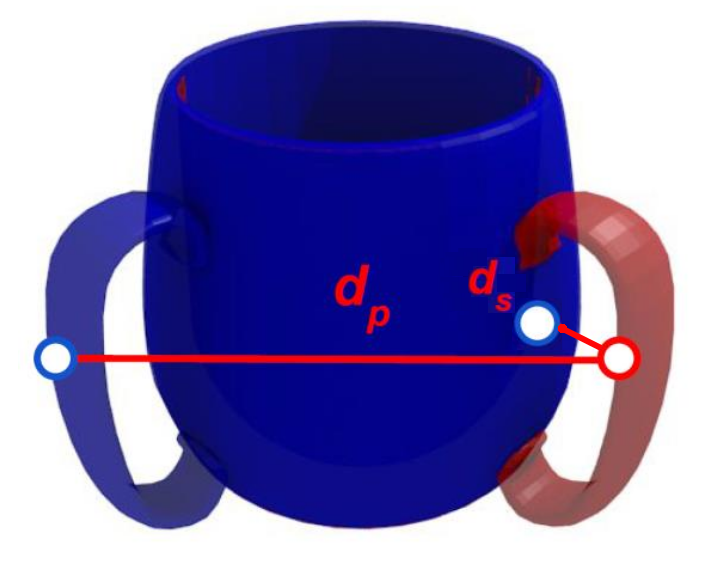
\includegraphics[width=0.5\textwidth]{figures/2_benchmarks_and_metrics/ds_vs_dp}
    \caption{\textbf{Maximum Distance ambiguities.} In this example it is clearly evident that the distance $d_p$ better reflects the misalignment w.r.t. the $d_s$ one.} 
    \label{fig:ds_vs_dp}
\end{figure}

\subsubsection{Visible Surface Distance (VSD)}\label{subsubsec:average_distance}
Do we need actually to perform the evaluation of the distance $d_p$ for all the points of the model $M$. It is actually a very computationally expensive task. That is why we now introduce the concept of \emph{Visible Surface}. The key-point here is to evaluate the distance only on the visible part of the model within the image:

\begin{equation}
    \label{eq:vis_surf_error}
    e_{VSD}(\hat{P}, \bar{P}; M, I, \delta, \tau) = avg_{p \in \hat{V} \cup \bar{V}} c(p, \hat{D}, \bar{D}, \tau)
\end{equation}

In Eq. \ref{eq:vis_surf_error}, $\hat{V}$ and $\bar{V}$ are the 2D masks of the visible surface of the projected models, with the ground truth pose $\hat{P}$ and the estimated pose $\bar{P}$ respectively. $\hat{D}$ and $\bar{D}$ are the \emph{distance images} obtained by rendering the two models in the camera reference frame. $\delta$ is a tolerance threshold used for the computation of the visibility masks, and $c(p, \hat{D}, \bar{D}, \tau) \in [0, 1]$ is the matching cost at pixel $p$:

\begin{equation}
    \label{eq:matching_cost_at_p}
    c(p, \hat{D}, \bar{D}, \tau) = \left\{
\begin{array}{c l}	
     \dfrac{d}{\tau} & if p \in \hat{V} \cap \bar{V} \wedge d > \tau \\
     1 & otherwise,
\end{array}\right.
\end{equation}

More in detail, in Eq. \ref{eq:matching_cost_at_p}, the distance image $d$ is given by:

\begin{equation}
    \label{eq:distance_image}
    d = |\hat{D}(p) - \bar{D}(p)|
\end{equation}

and it can be easily derived from the two depth images of the ground truth and the estimated poses respectively

In order to better understand the concept of visible surface, and the role of the visibility masks $\hat{V}$ and $\bar{V}$ in the equations \ref{eq:vis_surf_error} and \ref{eq:matching_cost_at_p}, let's take as example the mug depicted in Figure \ref{fig:visibility_mask_ex}.

\begin{figure}
    \centering
    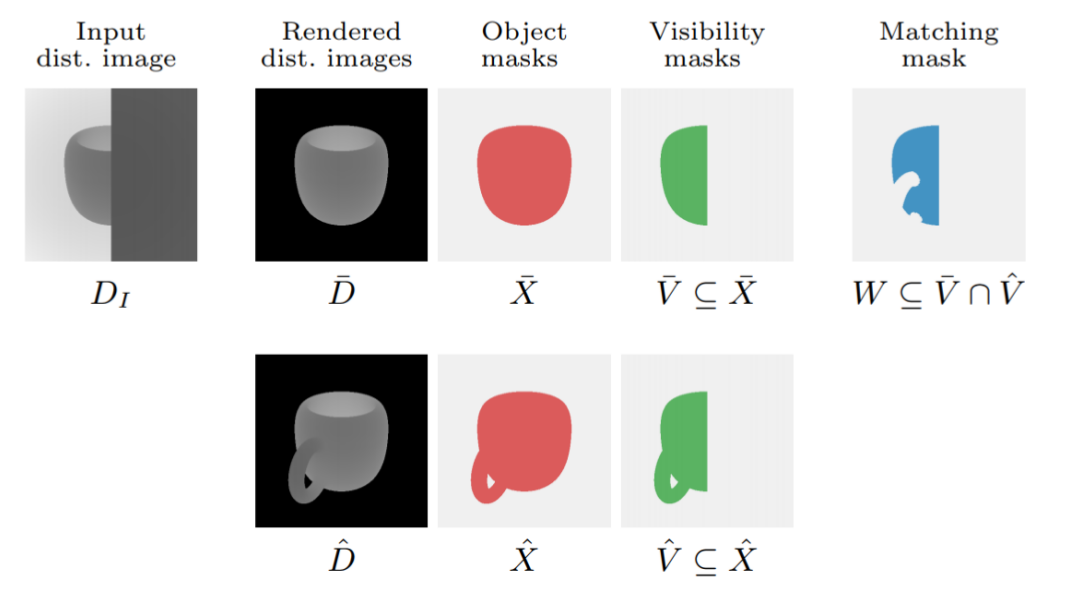
\includegraphics[width=0.8\textwidth]{figures/2_benchmarks_and_metrics/visibility_mask_ex}
    \caption{\textbf{Visibility Masks Example.} An example of how to compute the visibility mask for the mug in the image.}
    \label{fig:visibility_mask_ex}
\end{figure}

\section{Industrially oriented Datasets}\label{sec:datasets}
After having introduced and formulated the metrics used for comparing object detection and pose estimation measurements, we can now introduce some benchmark tools and data used for industrial applications. Typical settings are those with \emph{texture-less} objects, namely, objects that do not present any kind of texture. Given this property, object detectors and pose estimators can rely their estimations only on shape based approaches, without any sort of rbg texture based techniques.

Examples of texture-less datasets are the \emph{T-LESS} Dataset \cite{hodan2017tless} from the Center for Machine Perception of the Czech Technical University of Prague and the \emph{MVTec ITODD Dataset} \cite{mvtec2017itodd} from the same company that distributes the Halcon Libraries.

\begin{figure}
    \centering
    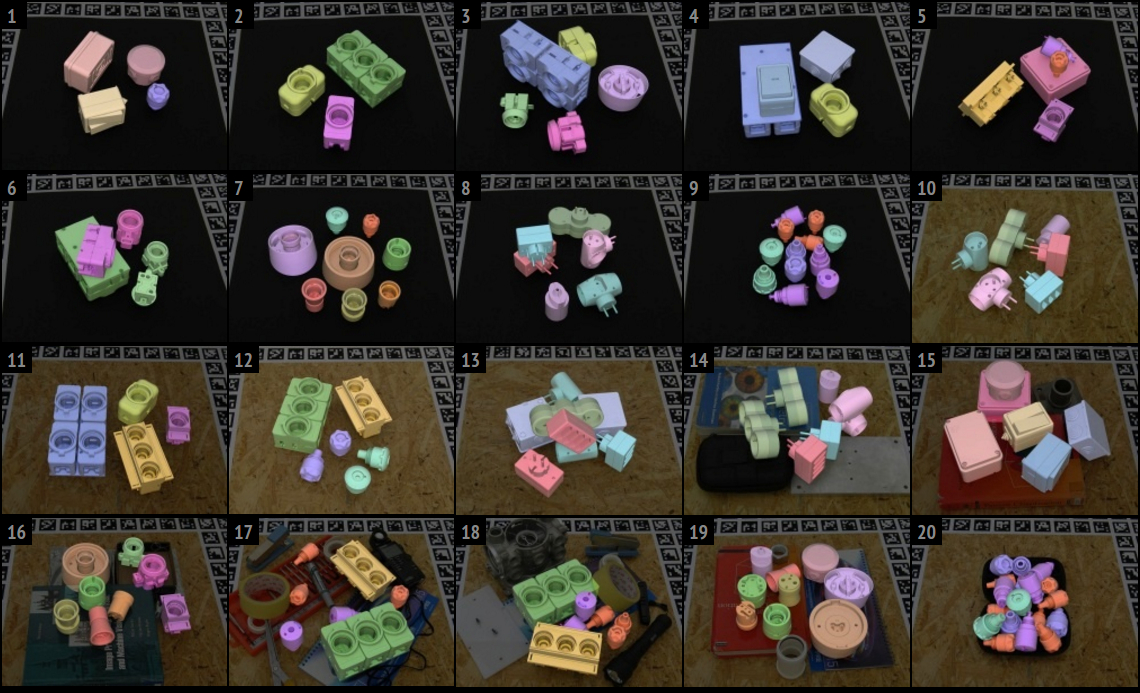
\includegraphics[width=0.8\textwidth]{figures/2_benchmarks_and_metrics/tless_ex_scenes}
    \caption{\textbf{T-LESS scenes examples.} A compact view of the scenes present in the T-LESS dataset.}
    \label{fig:tless_ex_scene}
\end{figure}

\subsection{T-LESS Dataset}\label{subsec:tless_dataset}
The T-LESS Dataset \cite{hodan2017tless}, has the name suggests, is a publicly available dataset\footnote{http://cmp.felk.cvut.cz/t-less/index.html} composed by thirty different texture-less objects. All the objects in the dataset are from the industrial scenario and do not present any particular feature, moreover, most of them are also very similar in shape and color.

The dataset is composed by training and test images, the former are represented by RGB and RGB-D images of multiple views of the single object, while the latter are composed by 21 test scenes where the objects are collected together in more cluttered and unstructurated forms. All the scenes, both training and test ones, have been acquired with a fixed sensor setup composed by the following RGB and RGB-D cameras:

\begin{itemize}
	\item Primesense Carmine 1.09 (Short Range) that provides registered RGB-D images with the following features: RGB:1280x1024 px, Depth:640x480 pixels;
	\item Microsoft Kinect v2 that provides images with registered depth with 1920x1080 pixels of resolution;
	\item Canon IXUS 950 IS high resolution camera that provides RGB images of 3264x2448 pixels of resolution.
\end{itemize}

All the three sensors have been mounted on a fixed structure and a rotating turntable with the objects on top has been built for positioning and rotating the training and test scenes. Examples of acquired scenes are in Figure \ref{fig:tless_ex_scene}.

In the T-LESS data packages also the CAD models of the objects are given to the public. In particular they released two different kind of CAD models:

\begin{itemize}
	\item Manually created CAD models;
	\item Automatically reconstructed CAD models.
\end{itemize}

%\begin{figure}
%    \centering
%    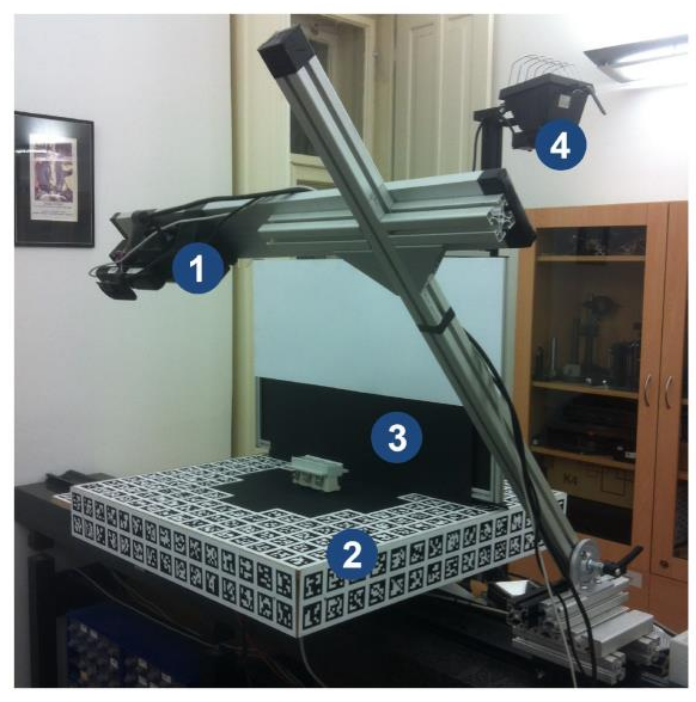
\includegraphics[width=0.9\textwidth]{figures/%2_benchmarks_and_metrics/tless_sensor_setup}
%    \caption{\textbf{T-LESS sensor setup.} The setup of the %sensors used during the acquisition of the T-LESS scenes. In the %picture}
%    \label{fig:tless_sensor_setup}
%\end{figure}

\begin{figure}
    \centering
    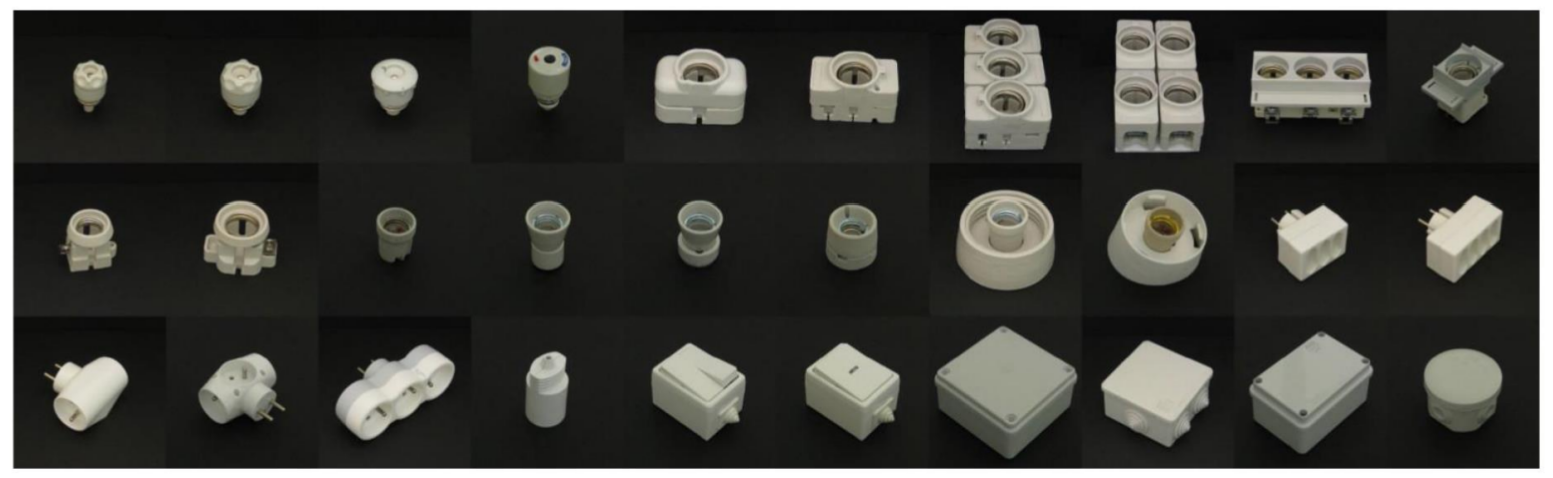
\includegraphics[width=0.9\textwidth]{figures/2_benchmarks_and_metrics/tless_objs_ex}
    \caption{\textbf{T-LESS Objects Samples.} A compact view of the thirty object classes present in the T-LESS dataset.}
    \label{fig:tless_objs_ex}
\end{figure}

All the objects presented in the T-LESS dataset are also shown here in Figure \ref{fig:tless_objs_ex}. As like as for our RAW dataset, they organized their objects in multiple scenes, 21 as already mentioned, classified by order of complexity: \emph{easy} and \emph{hard} objects scenes. Each scene has been accurately annotated, and all the objects in it have been localized following the approach explained below:

\begin{enumerate}
	\item A dense 3D model of the scene was reconstructed with the system from \cite{steinbrucker2014volumetric}. This was accomplished using all 504 RGB-D images of the scene along with the sensor poses estimated using the turntable markers;
	\item The CAD models were then manually aligned to the scene model;
	\item To increase accuracy, high-resolution images from Canon camera sensor were used to refine manually all the detected misalignments;
	\item The final poses were distributed to all the test images with the aid of the known camera-to-turntable coordinate transformations.
\end{enumerate}

\begin{figure}
    \centering
    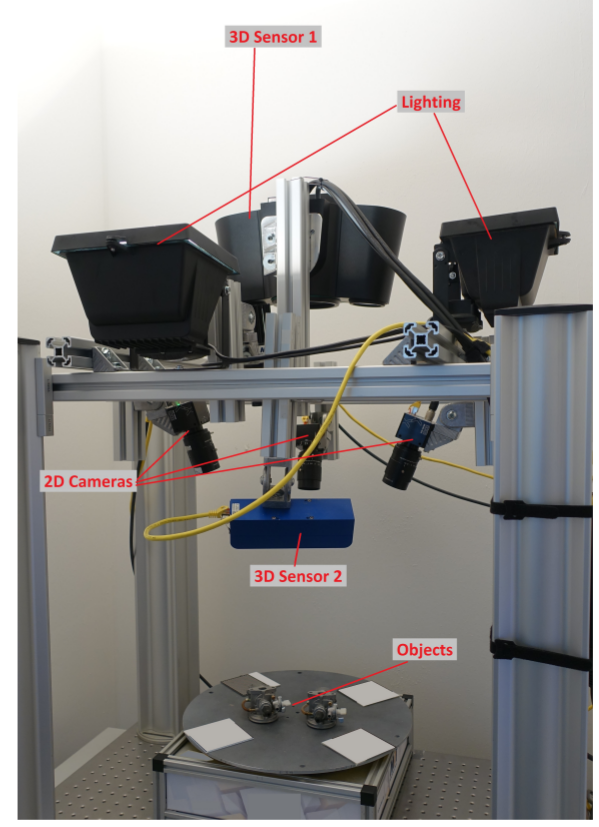
\includegraphics[height=0.4\textheight]{figures/2_benchmarks_and_metrics/itodd_sensor_setup}
    \caption{\textbf{MVTec ITODD Sensor Setup.} In the picture there is a compact view of the fixed sensor setup used for the acquisition of the MVTec ITODD dataset scenes.}
    \label{fig:itodd_sensor_setup}
\end{figure}

\subsection{MVTec ITODD}\label{subsec:mvtex_itodd}
MVTec Industrial 3D Object Detection Dataset, MVTec ITODD \cite{hodan20166DPoseEstimation} in code, is a public dataset for 3D object detection and pose estimation also related to industrial setups, like the previously mentioned T-LESS dataset. The dataset contains 28 object classes, disposed in 800 different scenes, all labeled with 3D rigid transformations with respect to the camera sensors.

The sensors used during the acquisition of the scenes are composed as follow:

\begin{itemize}
	\item High-Quality 3D sensor: a multi-shot 3D stereo sensor that provided both a depth image and a grayscale image with the same viewpoint of the previous one. This sensor also provided high-quality 3D reconstructed cloud of the scene by using multiple random projected patterns and a spacetime stereo approach for reconstructing the scene with an accuracy of around 100 $\mu m$;
	\item Low-Quality 3D sensor: very similar to the previous sensor but with a shorter baseline, a wider field of view and less shots per scene. Given those features, the 3D reconstructed scene is much more noisy than the previous one, with an accuracy of around 1-2 mm;
	\item 3 High.Resolution Cameras: they provided grayscale images, and the scenes where captured twice, one time with the random patterns and the last time without. 
\end{itemize}

In Figure \ref{fig:itodd_sensor_setup} there is a compact view of the fixed sensor setup used for the acquisition of the scenes in the dataset.

\begin{figure}
    \centering
    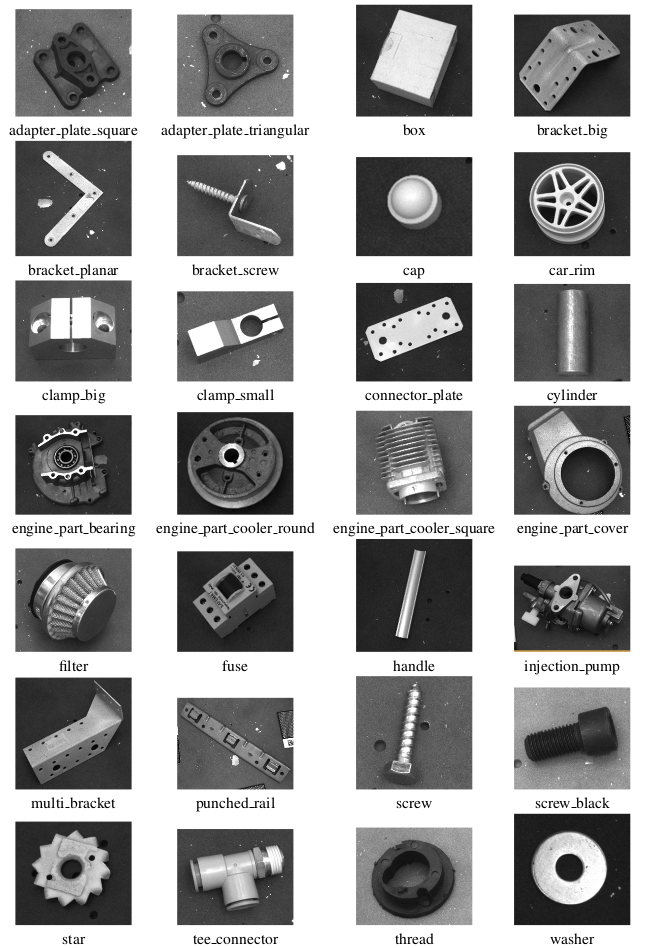
\includegraphics[width=0.8\textwidth]{figures/2_benchmarks_and_metrics/itodd_object_examples}
    \caption{\textbf{MVTec ITODD Object Classes.} All the 28 object classes of texture-less object used during the acquisition of the MVTec ITODD dataset scenes.}
    \label{fig:itodd_object_examples}
\end{figure}

As like as for the T-LESS dataset and the RAW Dataset that we are going to present in the next chapter, the object in the MVTec ITODD dataset are texture-less objects, that is for remarking again the high orientation to the industrial settings of these kind of works. All the object classes used in the MVTec ITODD dataset are depicted in Figure \ref{fig:itodd_object_examples}.
\newpage
\chapter{The RAW Dataset}\label{ch:benchmarks_and_metrics}
In this chapter the RAW dataset is going to be presented. This dataset has been produced as a requirement of the FlexSight\footnote{http://www.flexsight.eu/} project. FlexSight is a research project founded by the European Community's project ECHORD++\footnote{http://echord.eu/}.  This project involves three main partners: the Ro.Co.Co. Laboratory\footnote{http://www.dis.uniroma1.it/~labrococo/} of DIAG (Department of Computer, Control, and Management Engineering  Antonio Ruberti at Sapienza University of Rome), which provides expertise in software design and development for robotic perception applications; IT+Robotics\footnote{http://www.it-robotics.it/}, which provides expertise in the industrial robotics domain; and Robox\footnote{http://www.robox.it/en-US/}, a company specialized in the development of innovative hardware and software solutions for robotics and control systems. 

More details about the FlexSight project can be found in the Appendix \ref{apx:flexsight} of this thesis.

\section{RAW Dataset Features}\label{sec:raw_features}
As like as the previous datasets presented in sections \ref{subsec:mvtex_itodd} and \ref{subsec:tless_dataset} also the RAW Dataset has been built for industrial scenarios. The main scope of the RAW Dataset is to build a large and consistent test bed for texture-less object detection and localization algorithms. The name of the dataset is related to the RoboCup@Work competition, which more details are given in the Appendix \ref{apx:robocupatwork}, and it contains all the objects used in the robotic competition plus other objects from other past robotics events, such as the RoCKIn@Work\footnote{http://rockinrobotchallenge.eu/} (Robot Competitions Kick Innovation in Cognitive Systems and Robotics) and ERL\footnote{https://www.eu-robotics.net/robotics\_league/index.html} (European Robotics League). 

As already mentioned, all the objects present in the dataset are texture-less objects and are inspired to the industrial settings, e.g. parts of a motor, bearings, nuts, motor axis and others. A compact view of all the objects present in the dataset is given in Figure \ref{fig:raw_obj_examples}, and the complete list of objects with their specific name and class is reported in Table \ref{tab:raw_objs_list}.

\begin{table}
    \centering
    \begin{tabular}{| l | l | l |}
    \hline
    \textbf{Name} & \textbf{Class} & \textbf{Description} \\ \hline
    F20\_20\_B & 0 & Black small aluminium profile \\
    F20\_20\_G & 1 & Gray small aluminium profile \\
    M20 & 2 & Small nut \\
    M20\_100 & 3 & Heavy large screw \\
    M30 & 4 & Big nut \\
    R20 & 5 & Plastic tube with shaped borders \\
    S40\_40\_B & 6 & Black large aluminium profile \\
    S40\_40\_G & 7 & Gray large aluminium profile \\
    V20 & 8 & Plastic tube without shaped borders \\
    Bearing\_box & 9 & Small motor box for bearings \\
    Bearing\_box\_B & 10 & Small motor box for bearings (Type B) \\
    Motor & 11 & Black plastic reconstruction of a motor \\
    Axis & 12 & Aluminium motor axis \\
    Distance\_tube & 13 & Small aluminium ring \\
    Bearing & 14 & Real bearing for motors \\
    Cover\_plate\_NOHOLE & 15 & Thin aluminium plate with hole \\
    Cover\_plate\_HOLE & 16 & Thin aluminium plate without hole \\
    Cover\_plate\_BOX & 17 & Black plastic box for cover plates \\
    Bearing\_box\_BOX & 18 & Black plastic box for bearing boxes \\
    \hline
    \end{tabular}
    \caption{\textbf{The RAW Dataset Objects.} In this table is reported the list of all the objects present in the RAW dataset, with their name and class.}
    \label{tab:raw_objs_list}
\end{table}

\begin{figure}
    \centering
    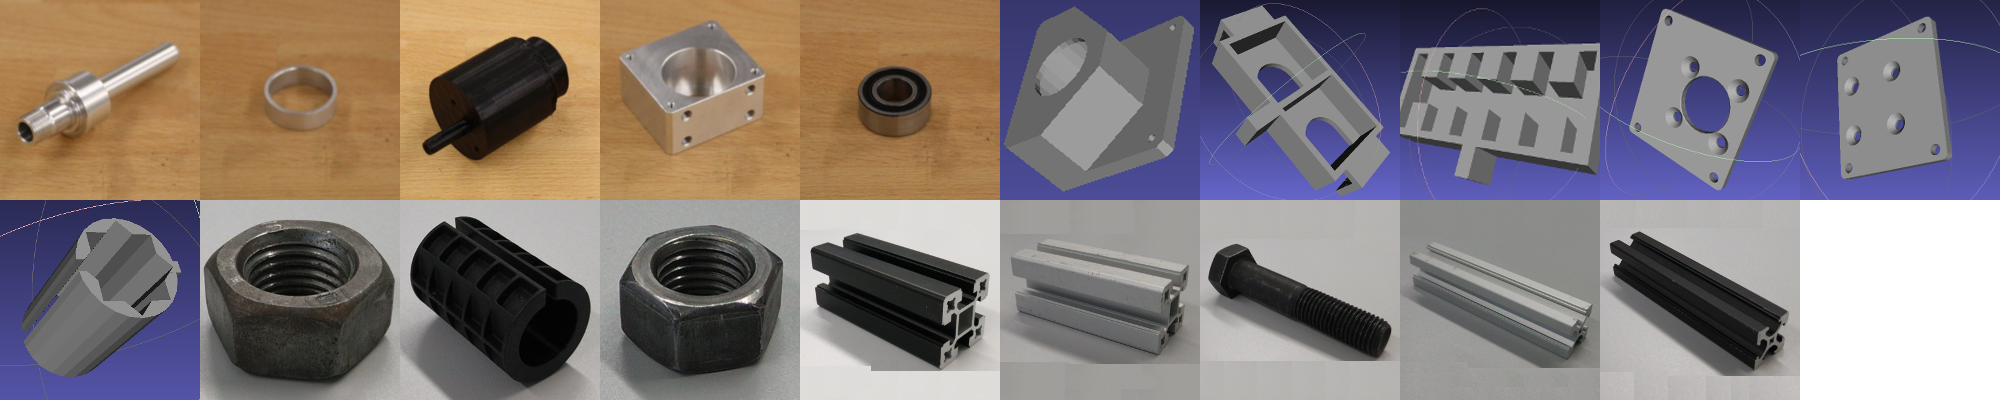
\includegraphics[width=0.9\textwidth]{figures/3_raw_dataset/raw_obj_examples}
    \caption{\textbf{RAW Dataset Objects.} A compact view of all the 19 classes of objects present in the RAW Dataset.}
    \label{fig:raw_obj_examples}
\end{figure}

The main features of this dataset are the following:
\begin{itemize}
	\item \textbf{19 indutry relevant objects}: no discriminative color, no texture, often similar in shape;
	\item \textbf{3 different sensors}: FlexSight sensor, Microsoft Kinect2, Intel RealSense SR-300;
	\item \textbf{Test images (7K from each sensor)}: originated from 15 test scenes. The scene complexity varies from simple scenes with several isolated objects to very challenging ones with multiple object instances and a high amount of clutter and occlusion. Images include: RGB and Depth for Kinect2 and RealSense SR-300; 2 grey-scale images (with and without projected laser pattern) for the FlexSight sensor;
	\item \textbf{19 object 3D CAD models}: all the objects have a specific 3D CAD model.
\end{itemize}

Each image of the dataset comes with ground truth estimate of all the objects present in the scene. The full 3D position in space, rotation plus translation with respect to the camera frame, has been annotated with a specific protocol that involved both manually intervention of the user by means of our own developed labeling tool and some other automatic procedures for propagating the pose in a given reference frame to all the other images of the dataset.

\begin{figure}
    \centering
    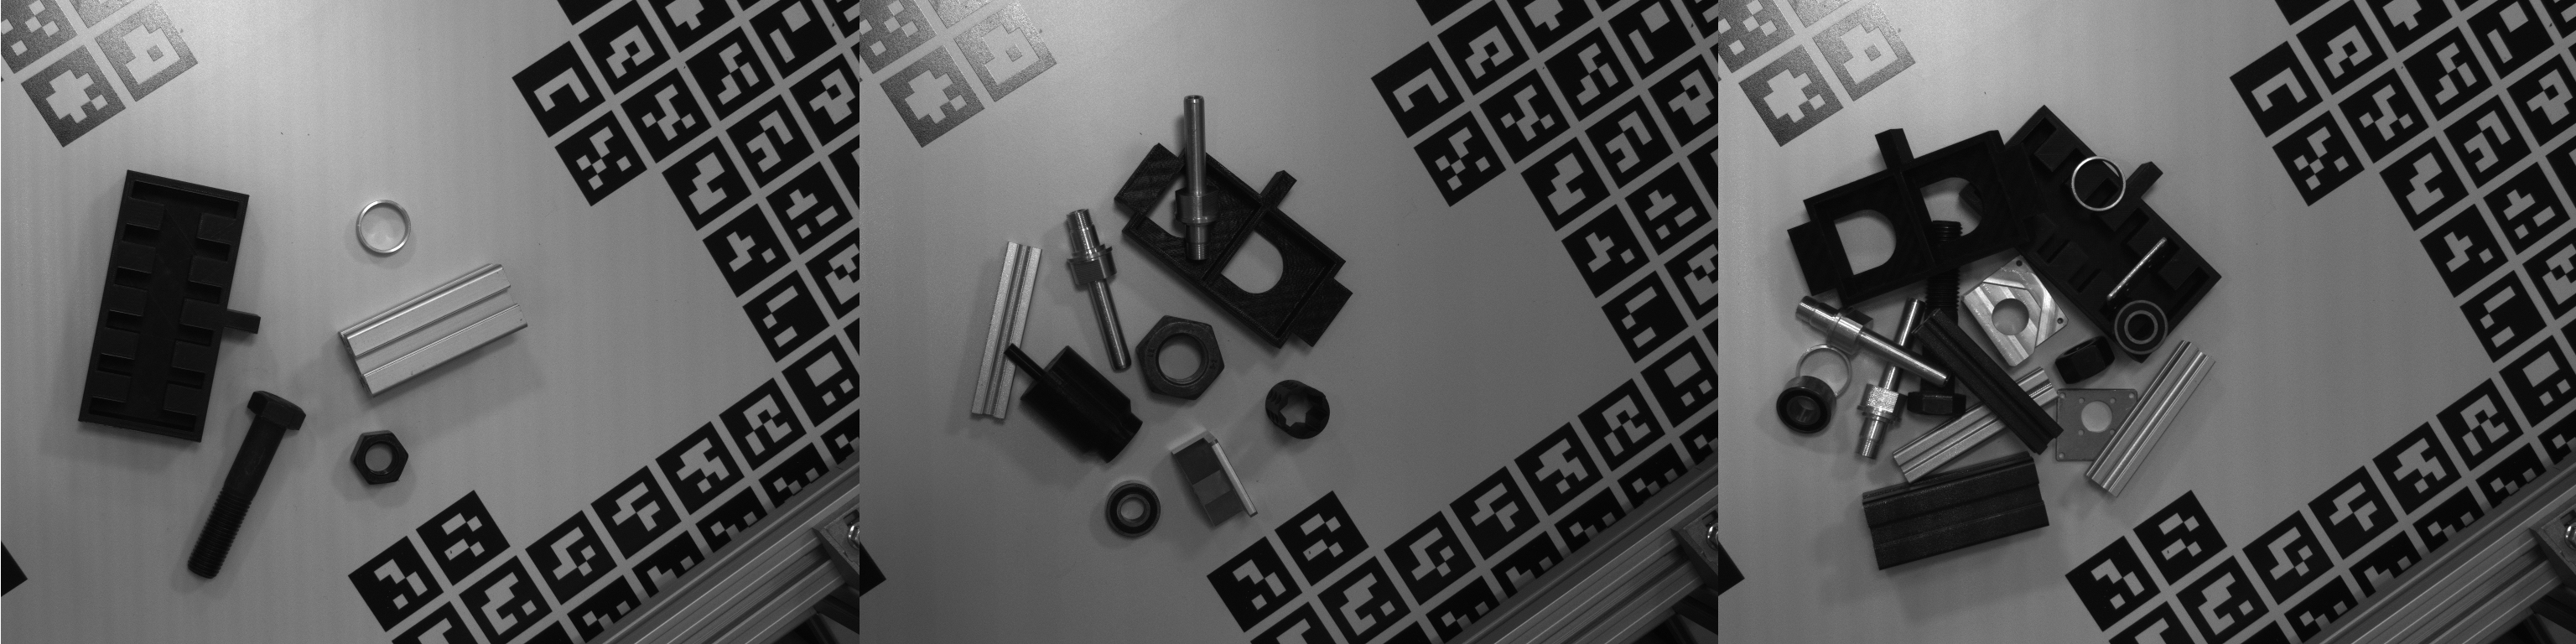
\includegraphics[width=0.9\textwidth]{figures/3_raw_dataset/easy_medium_hard_scene}
    \caption{\textbf{RAW Dataset Scenes Comparison.} From left to right: easy scene, medium scene and hard scene. All the images refers to the camera left of the FlexSight sensor and are without the projected laser pattern.}
    \label{fig:easy_medium_hard_scene}
\end{figure}

\section{Details of the Scenes}\label{sec:raw_scenes_details}
As already anticipated, the RAW Dataset comes with 15 different scenes. In particular, those scenes are aggregated in three different categories: \emph{easy}, \emph{medium} and \emph{hard}. This categorization depends on the level of complexity of the disposition of the objects in the scenes. An example of easy medium and hard scene comparison is given in Figure \ref{fig:easy_medium_hard_scene}. Moreover, easy scenes does not contain any occlusion or overlapping of the objects, while medium and hard scenes do.

Each scene is composed as follow:

\begin{itemize}
	\item \textbf{FlexSight Sensor Data}: 465 images, both for camera left and camera right of the sensor. Each image has been acquired with and without the projected laser pattern (See Figure \ref{fig:flexsight_laser_no_laser_ex}).
	\item \textbf{Microsoft Kinect 2}: 465 rgb-d images. We provide both rgb and depth image, together with the automatic generated registered pointcloud.
	\item \textbf{Intel Realsense SR300}: 465 rgb-d images. For the Intel Realsense SR300 only rgb and depth images are provided.
\end{itemize}

\begin{figure}
    \centering
    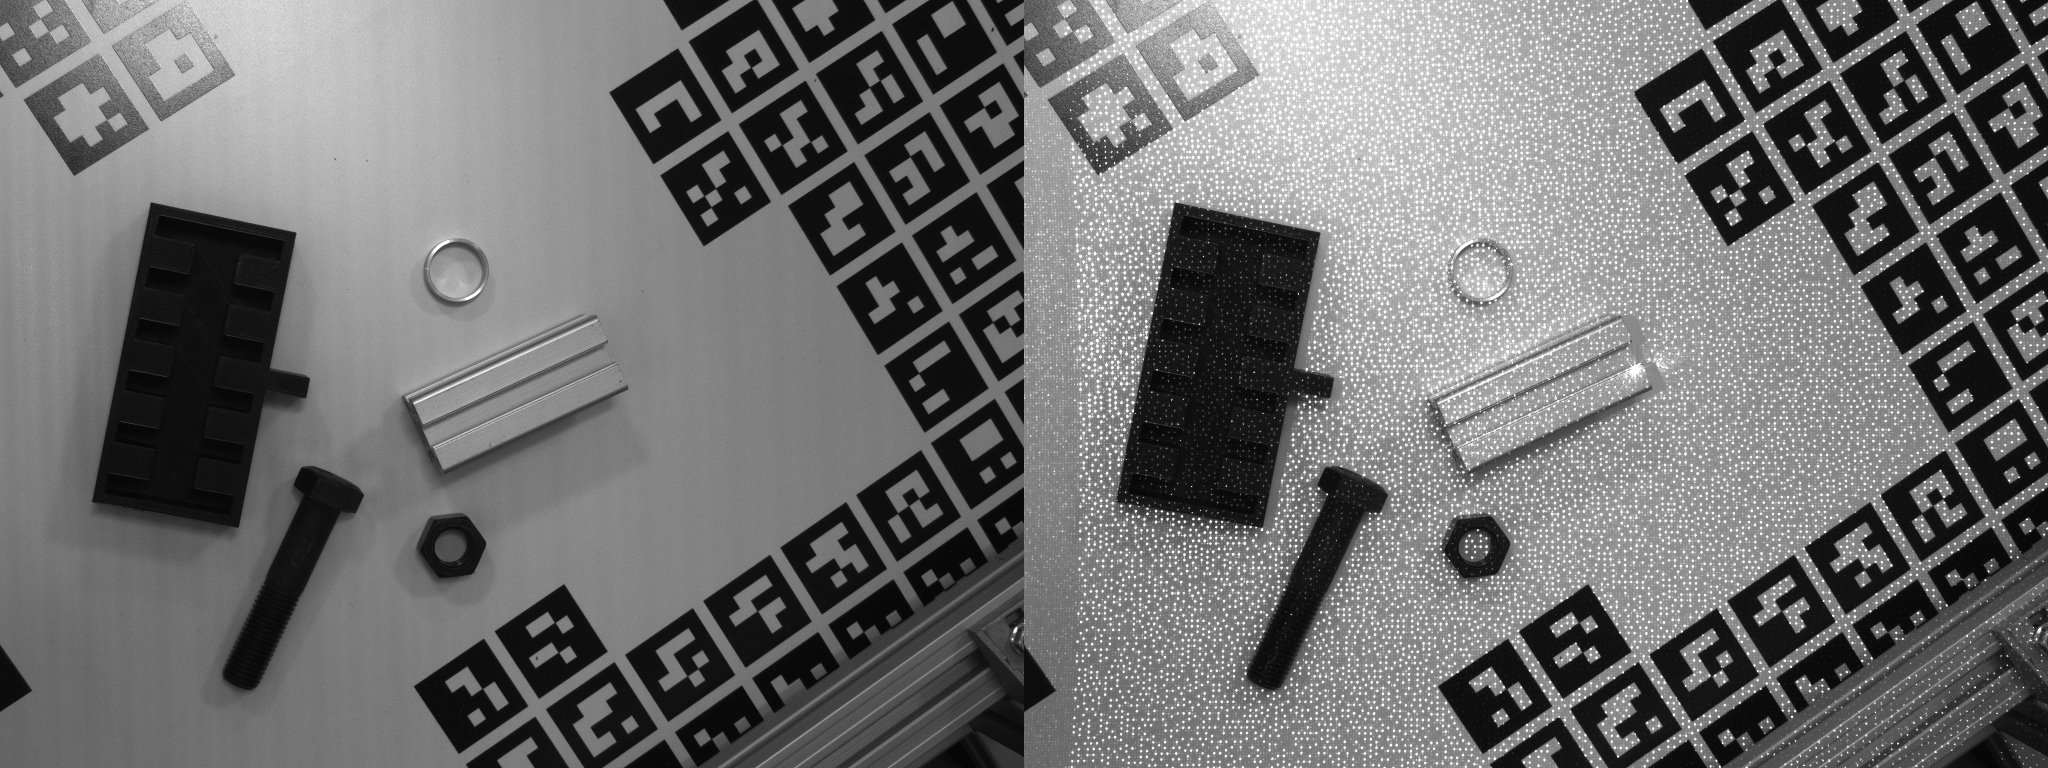
\includegraphics[width=0.9\textwidth]{figures/3_raw_dataset/flexsight_laser_no_laser_ex}
    \caption{\textbf{FlexSight Sensor Acquisition (with and without laser pattern).} On the left the FlexSight Sensor image acquired without projected laser pattern, on the right with projected laser pattern.}
    \label{fig:flexsight_laser_no_laser_ex}
\end{figure}

\section{Setup and Sensors}\label{sec:raw_setup_and_sensors}
As already mentioned in the introduction if this chapter, the RAW Dataset has been acquired in fulfillment of the data acquisition requirement of the FlexSight project. For this scope, a completely new and custom robot-sensors setup has been built in collaboration with the two other partners of the project, IT+Robotics and Robox. This setup consists in a custom built cell with a robotic manipulator inside, which has the experimental sensor mounted at its end-effector. A 3D model view of the robotic cell is given in Figure \ref{fig:raw_cell_example}.

In the following sections the robotic arm and all the sensors will be explained in detail.

\begin{figure}
    \centering
    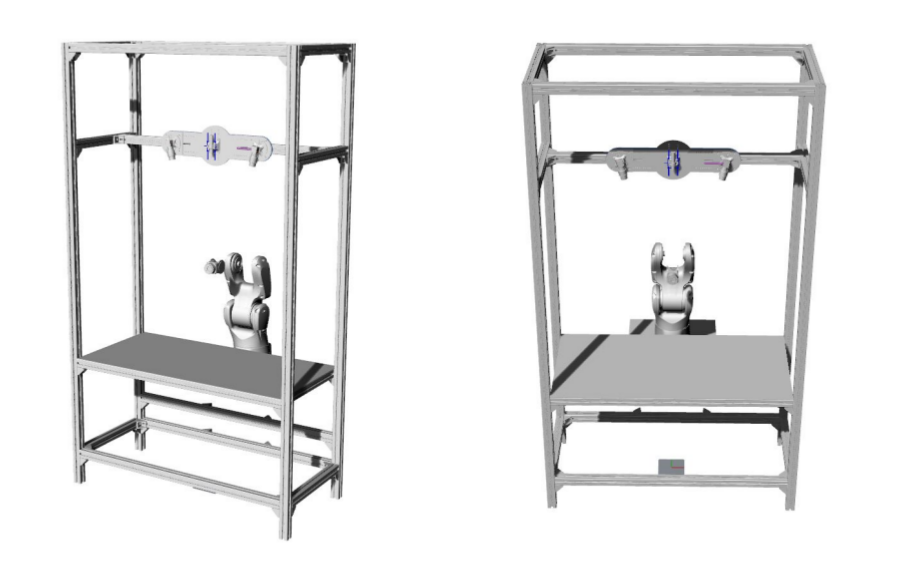
\includegraphics[width=0.9\textwidth]{figures/3_raw_dataset/raw_cell_example}
    \caption{\textbf{FlexSight Robotic Cell 3D Model View.} A 3D reconstruction of the custom robotic cell developed and built for the RAW Dataset acquisition. The figure just reports the robotic cell with the first prototype of the FlexSight sensor mounted on the top and a fake robotic arm as placeholder for the real one.}
    \label{fig:raw_cell_example}
\end{figure}

\subsection{The Robotic Arm}\label{subsec:raw_setup_robot}
The robotic arm used for the acquisition of the RAW Dataset is a 6 d.o.f. robotic manipulator. It has been provided by Robox as contribution to the FlexSight project.The company also provided their own control system with which we interfaced via serial communication for positioning and sending commands to the robot during the acquisition procedure. A picture of the robotic manipulator is given in Figure \ref{fig:raw_robot_example}.

\begin{figure}
    \centering
    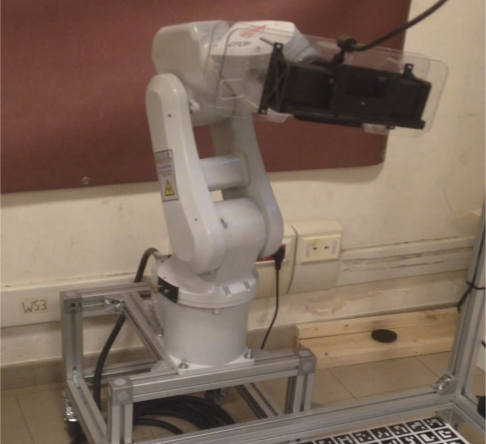
\includegraphics[width=0.8\textwidth]{figures/3_raw_dataset/raw_robot_example}
    \caption{\textbf{FlexSight Robotic Manipulator}. In the picture, the 6 d.o.f. robotic manipulator used for the acquisition of the RAW Dataset scenes.}
    \label{fig:raw_robot_example}
\end{figure}

\subsection{The FlexSight Sensor}\label{subsec:raw_setup_fss}
The main contribution of this thesis project was the acquisition of a novel dataset with a novel sensor, that provides both high-resolution images for active and passive stereo vision. This sensor, we named it FlexSight Sensor is composed by 2 main components:

\begin{itemize}
	\item A stereo camera setup, composed by two high resolution grayscale cameras. Each camera provides high-resolution grayscale images, in particular: \emph{2048x1536 px} of resolution.
	\item A pseudo-random laser projector. This was involved to achieve active stereo capabilities.
\end{itemize}

A detailed view of the FlexSight sensor is given in Figure \ref{fig:fs_sensor_0}. The sensor has been mounted on a custom support at the end-effector of the robotic manipulator. Moreover it presents a \emph{Arduino MEGA} controller used for triggering the two cameras and the laser projector in the same moment in order to achieve precise and accurate image acquisition. Both the cameras and the laser projector have been powered by 5V DC adapter which provides stabilized and regular DC current to each device.

\begin{figure}
    \centering
    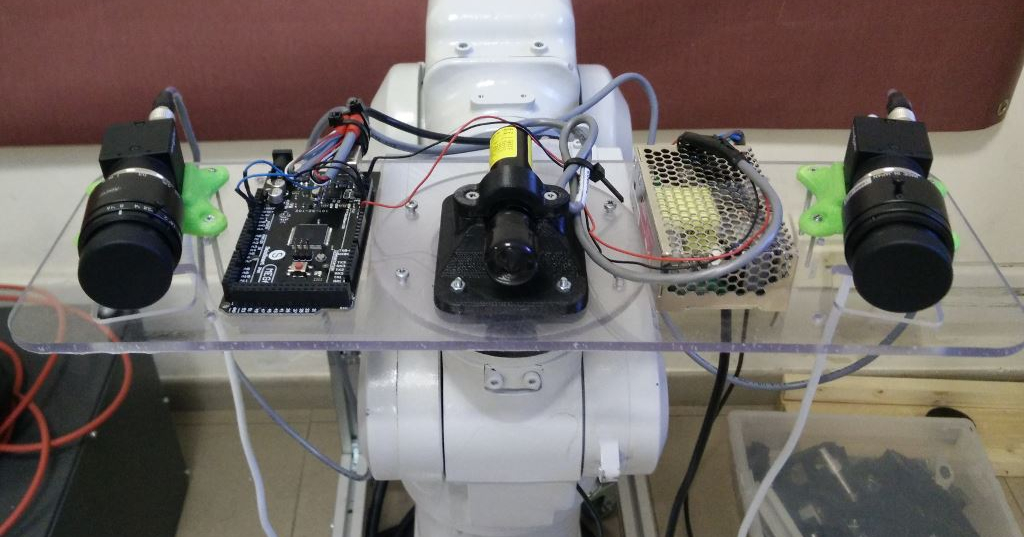
\includegraphics[width=0.8\textwidth]{figures/3_raw_dataset/fs_sensor_0}
    \caption{\textbf{FlexSight Sensor Detail}. From left to right: right high-resolution pointgray camera, arduino controller, pseudo-random laser projector, AC adapter, left high-resolution pointgray camera.}
    \label{fig:fs_sensor_0}
\end{figure}

\subsection{Microsoft Kinect 2 and Intel Realsense SR300}\label{subsec:raw_setup_kin&realsense}
On top of the FlexSight sensor, two commercially available 3D sensors have been mounted, namely a Microsoft Kinect 2 RGB-D sensor and a Intel Realsense SR300. Both the commercial sensors provided already registered depth and rgb images at low and high resolution respectively.

\begin{itemize}
	\item \textbf{RGB images}: \emph{1920x1080 px} for both the sensors.
	\item \textbf{Depth images}: \emph{512x424 px} for Microsoft Kinect 2 and \emph{640x480} for the Intel Realsense SR300.
\end{itemize}

Moreover, the two sensors have been chosen because they provide different features and can be of major interests for other commercial and common usages. In particular, the Intel Realsense SR300 is a so called \emph{short range} sensor, in the sense that its depth estimation is accurately working in short ranges, namely $0.2m$ to $1.5m$. While the Microsoft Kinect 2 provides wider range, namely $0.8m$ to $4.5m$.

\section{Acquisition Procedure}\label{sec:raw_acquisition_procedure}
To do ...

\section{Ground Truth Estimation Protocol}\label{sec:ground_truth_estim}
To do ...

\subsection{Labelling tool}\label{subsec:raw_labeltool}
To do ...

\subsection{Pose Propagation Pipeline}\label{subsec:pose_propagation}
To do ...
\newpage
\chapter{Experiments}\label{ch:experiments}
In this chapter we will exploit in detail some experiments performed over the RAW Dataset presented in Chatper \ref{ch:raw_dataset}. In particular we will first focus on some object detection experiments performed both with standard shape based approaches as described in Sec. \ref{subsec:template_matching} and deep learning based approaches as described in Sec. \ref{subsec:dl_obj_detection}. Moreover, we will exploit the results of our implementation of the SGM algorithm described in Sec. \ref{subsec:semiglobalmatching} comparing its results with the ground truth depth image created by reconstructing the 3D scene with the ground truth objects pose obtained with the labeling procedure described in Sec. \ref{sec:ground_truth_estim}.

%\section{Region Proposal}\label{sec:exp_region_proposal}
%To do ...

\section{Object Detection}\label{sec:exp_object_detection}
As aleady inoduced in Sec. \ref{sec:objectdetection}, object detection is basically the task of computing the 2D boinging box of a given object within an image. Bounding box is essentially a portion of the image that contains the object. Such basic information is extremely important in robotic perception, especially in robotic vision, where the ability to detect objects in different situations is a crucial point. Our tests basically rely on testing the performances of two different kind of approaches, namely shape based and deep learning.

The tests have been performed on a subset of the RAW Dataset, since the availability of the ground truth for the entire dataset has not been achieved yet, moreover it is not part of the scope of this work. The subset of the RAW Dataset is anyway enough large to permit consistent and coherent statistical evaluations, and it is composed as follows:

\begin{itemize}
	\item \textbf{2 complete scenes}: the tests have been performed using just the first two scenes of the dataset, and just with respect to the data obtained from the experimental FlexSight Sensor, as its performance evaluation is a consistent and important part of the FlexSight project (See Appendix \ref{apx:flexsight});
	\item \textbf{Almost 4 thousand of images}: the two scenes contains both camera left and camera right of the FlexSight Sensor, both with and without projected laser pattern;
	\item \textbf{All the images are labeled}: all the considered images have are accompanied with the relative ground truth 3D position of each object and the relative bounding box as well;
	\item \textbf{5 Different Object Classes}: the involved images only contain 5 object classes of the RAW Dataset, namely: \emph{Distance\_tube}, \emph{M20}, \emph{M20\_100}, \emph{Cover\_plate\_BOX}, \emph{S40\_40\_G};
	\item \textbf{Synthetic data generation}: for the deep learning approaches, data augmentation has been employed. In particular we will see in the following subsections how we trained the YOLO deep neural network described in Sec. \ref{subsec:dl_obj_detection} with 2 different version of the RAW Dataset subset, namely the first is the original one and the second is a synthetic version of it.
\end{itemize}

The results wiil be organized by class of the object and will be expressed in terms of IoU accuracy over the detected bounding box.

\subsection{Shape Based Approach Results - Halcon object detection}\label{subsec:halcon_obj_det_results}
\subsubsection{Experiment Details}
In this experiment, we performed both object localization and detection since the core of the object detection pipeline of the Halcon libs is essentially based on 3D object localization on 2D images, then given the 3D position of the object w.r.t. the camera frame, it is projected onto the 2D image and the bounding box of the object is extracted. Examples of this procedure is given in \figref{fig:iou_example}. Moreover, given the highly customization level that those library has, we investigated object detection performances by considering multiple settings:

\begin{itemize}
	\item \textbf{Single object candidate detection}: Only the object with the highest score is considered;
	\item \textbf{Multiple object candidates detection}: We analyzed both the performances using in sequence: \emph{5 candidates}, \emph{4 candidates}, \emph{3 candidates} and \emph{2 candidates}.
\end{itemize}

\begin{figure}
    \centering
    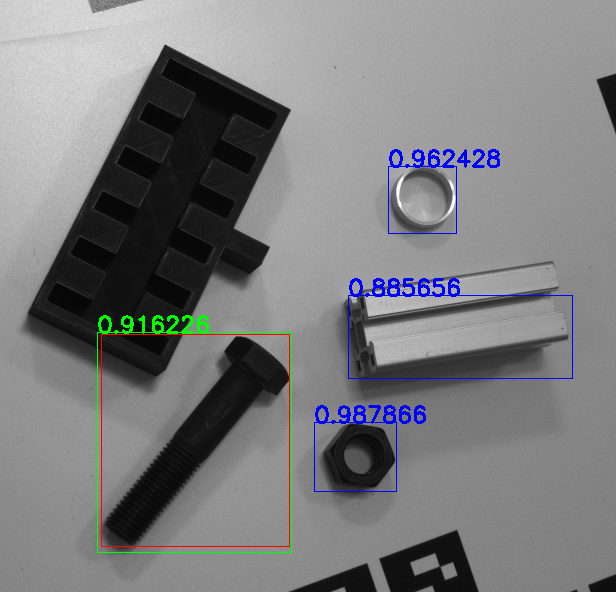
\includegraphics[width=0.8\textwidth]{figures/4_experiments/m20_100_halcon_detection_problems}
    \caption{\textbf{Best Candidate Problems with Halcon Libraries}. The picture depicts an example of erroneous best candidate detection. The candidate that actually refers to the real M20\_100 object is not the one with the highest score. In a single candidate approach the detection would have failed.}
    \label{fig:m20_100_halcon_detection_problems}
\end{figure}

\subsubsection{Experiment Results}
As already anticipated, each result will be presented differentiating for each class of the considered objects. The \tabref{tab:big_table_results} show the accuracy results in terms of Intersection over Union (IoU) for each of the involved object, look at the section referred to Shape Based Approach.

As expected, the performances slightly increase when including in the search procedure the highest number of candidates. That is essentially due to the fact that not always the first best candidate, namely the object with the highest score, is exactly the object that we are looking for. If we compare more than one candidate with the ground truth bounding box we find that for some classes of objects, like the \emph{M20\_100}, only when we consider 5 candidates we achieve to detect the actual object, and even in such cases, the one that has the highest score is not the right object (See. \figref{fig:m20_100_halcon_detection_problems} for a better visualization of the described problem).

\begin{table}[ht!]
 \centering

   \begin{tabular}{ llllllll }
   &\multicolumn{5}{c}{ \textbf{Shape Based} } &\multicolumn{2}{c}{ \textbf{Deep Learning} }\\
   \cmidrule(lr){2-6} \cmidrule(lr){7-8}
   \textbf{Obj Class} & \emph{1Cand} & \emph{2Cand} & \emph{3Cand} &\emph{4Cand} & \emph{5Cand} & $YOLO_O$ & $YOLO_S$\\
   \cmidrule(lr){1-8}   
   \emph{Distance\_tube} & 0.862 & 0.862 & 0.862 & 0.862 & 0.862 & \cellcolor{gray!25}0.897 & 0.825 \\ 
   \emph{M20} & 0.744 & 0.744 & 0.746 & 0.746 & 0.746 & \cellcolor{gray!25}0.901 & 0.816 \\ 
   \emph{M20\_100} & 0.000 & 0.000 & 0.475 & 0.475 & 0.797 & \cellcolor{gray!25}0.944 & 0.890 \\
   \emph{Cover\_plate\_BOX} & 0.799 & 0.799 & 0.799 & 0.799 & 0.799 & \cellcolor{gray!25}0.954 & 0.921 \\
   \emph{S40\_40\_G} & 0.809 & 0.809 & 0.809 & 0.809 & 0.809 & \cellcolor{gray!25}0.939 & 0.829 \\
%   \vspace{0.025cm} \\
%   \cline{1-8} \\
   \end{tabular} 
   \caption{\textbf{IoU Average results}: the table reports the results in terms of IoU Average (Intersection over Union Average) of all the tested methods. Results are reported by object class organized in columns by Shape Based Approach and Deep Learning Approach. Shape Based Approach results are reported by number of candidates used for the detection.}
 \label{tab:big_table_results}
\end{table}

%\begin{table}[!hbt]
%\parbox{.45\linewidth}{
%	\centering
%    \begin{tabular}{| l | l |}
%    \hline
%    \textbf{Experiment Type} & \textbf{IoU Average} \\ \hline
%    \emph{5 candidates} & 0.86190 \\
%    \emph{4 candidates} & 0.86190 \\
%    \emph{3 candidates} & 0.86190 \\
%    \emph{2 candidates} & 0.86190 \\
%    \emph{1 candidate} & 0.86190 \\
%    \hline
%    \end{tabular}
%    \caption{\textbf{Halcon IoU avg. scores on Distance\_tube object.}}
%    \label{tab:halcon_distance_tube_results}
%}
%\hfill
%\parbox{.45\linewidth}{
%	\centering
%    \begin{tabular}{| l | l |}
%    \hline
%    \textbf{Experiment Type} & \textbf{IoU Average} \\ \hline
%    \emph{5 candidates} & \textbf{0.74614} \\
%    \emph{4 candidates} & \textbf{0.74614} \\
%    \emph{3 candidates} & \textbf{0.74614} \\
%    \emph{2 candidates} & 0.74418\\
%    \emph{1 candidate} & 0.74418\\
%    \hline
%    \end{tabular}
%    \caption{\textbf{Halcon IoU avg. scores on M20 object.}}
%    \label{tab:halcon_M20_results}
%}
%\end{table}
%
%\begin{table}[!hbt]
%\parbox{.45\linewidth}{
%	\centering
%    \begin{tabular}{| l | l |}
%    \hline
%    \textbf{Experiment Type} & \textbf{IoU Average} \\ \hline
%    \emph{5 candidates} & \textbf{0.79750} \\
%    \emph{4 candidates} & 0.47585 \\
%    \emph{3 candidates} & 0.47585 \\
%    \emph{2 candidates} & 0.00000 \\
%    \emph{1 candidate} & 0.00000 \\
%    \hline
%    \end{tabular}
%    \caption{\textbf{Halcon IoU avg. scores on M20\_100 object.}}
%    \label{tab:halcon_M20_100_results}
%}
%\hfill
%\parbox{.45\linewidth}{
%	\centering
%    \begin{tabular}{| l | l |}
%    \hline
%    \textbf{Experiment Type} & \textbf{IoU Average} \\ \hline
%    \emph{5 candidates} & \textbf{0.79978} \\
%    \emph{4 candidates} & \textbf{0.79978} \\
%    \emph{3 candidates} & \textbf{0.79978} \\
%    \emph{2 candidates} & \textbf{0.79978} \\
%    \emph{1 candidate} & 0.12 \\
%    \hline
%    \end{tabular}
%    \caption{\textbf{Halcon IoU avg. scores on Cover\_plate\_BOX object.}}
%    \label{tab:halcon_Cover_plate_BOX_results}
%}
%\end{table}
%
%\begin{table}[!hbt]
%	\centering
%    \begin{tabular}{| l | l |}
%    \hline
%    \textbf{Experiment Type} & \textbf{IoU Average} \\ \hline
%    \emph{5 candidates} & 0.80922 \\
%    \emph{4 candidates} & 0.80922 \\
%    \emph{3 candidates} & 0.80922 \\
%    \emph{2 candidates} & 0.80922 \\
%    \emph{1 candidate} & 0.80922 \\
%    \hline
%    \end{tabular}
%    \caption{\textbf{Halcon IoU avg. scores on S40\_40\_G object.}}
%    \label{tab:halcon_S40_40_G_results}
%\end{table}

\subsection{Deep Learning Approach Results - YOLO}\label{subsec:yolo_obj_det_results}
\subsubsection{Experiment Details}
Deep learning is become one of the prominent and more prolific area of research in the last decade, and latest techniques and developments have actually now reached the state-of-the-art in many tasks. Object detection is one of them. That is why we wished to test some of those techniques, e.g. YOLO deep neural network, and compare its performance w.r.t. the technique used in the last experiment. In this experiment we are going to show multiple results of YOLO object detection capabilities and explain how we achieved higher levels of IoU Avg. detection rate w.r.t. the Halcon libraries.

The experiment has been conducted using almost the very same settings of the previous experiment, with just few modifications in order to be compliant with this totally different approach. In particular, given the data driven nature of this approach we must subdivide the dataset in two different sets: \emph{training set}, \emph{evaluation set}. In particular we used $95\%$ of the initial subset as training set, and the remaining $5\%$ as validation set. The high disparity among the two set sizes is simply because such approaches need lot of data in order to be trained successfully, that is we gave almost all the subset to the training set. The validation set at the end is big enough to obtain reliable results ($\sim$ 100 images). From now on, we will refer to this version of the dataset as \emph{$YOLO_O$}, as it is directly built from the original RAW Dataset, and just adapted to the YOLO format. The same acronym will be given to the related network as well.

\begin{table}
	\centering
    \begin{tabular}{| l | l |}
    \hline
    \textbf{Parameter} & \textbf{Value} \\ \hline
    \emph{batch size} & 64 \\
	\emph{height} & 416 \\
	\emph{momentum} & 0.9 \\
	\emph{decay} & 0.0005 \\
	\emph{learning rate} & 0.0001 \\
	\emph{max batches} & 15000 \\
	\emph{policy} & steps \\
	\emph{steps} & 100, 8000, 10500 \\
    \hline
    \end{tabular}
    \caption{\textbf{$YOLO_O$ training parameters.} In the table are reported the most significant parameters that we tuned in order to train the $YOLO_O$ network. All the others are assumed as with their default value.}
    \label{tab:YOLO_standard_training_params}
\end{table}

The training of the $YOLO_O$ network has been conducted using the set of parameters given in \tabref{tab:YOLO_standard_training_params}. With the very same set of parameters we performed another train of the YOLO network. In particular we used a \emph{synthetic} version of the RAW Dataset, from now on we will refer to it as $YOLO_S$, built by manipulating the same training images used for $YOLO_O$'s training. The basic idea was to change the background of all the images with random images downloaded from the publicly available set of images at the following site: \url{https://snippets.khromov.se/stock-photo-archive-zip-77-images/}. Some example of images realized with such technique, are given in \figref{fig:synthetic_dataset_ex}.

\begin{figure}
    \centering
    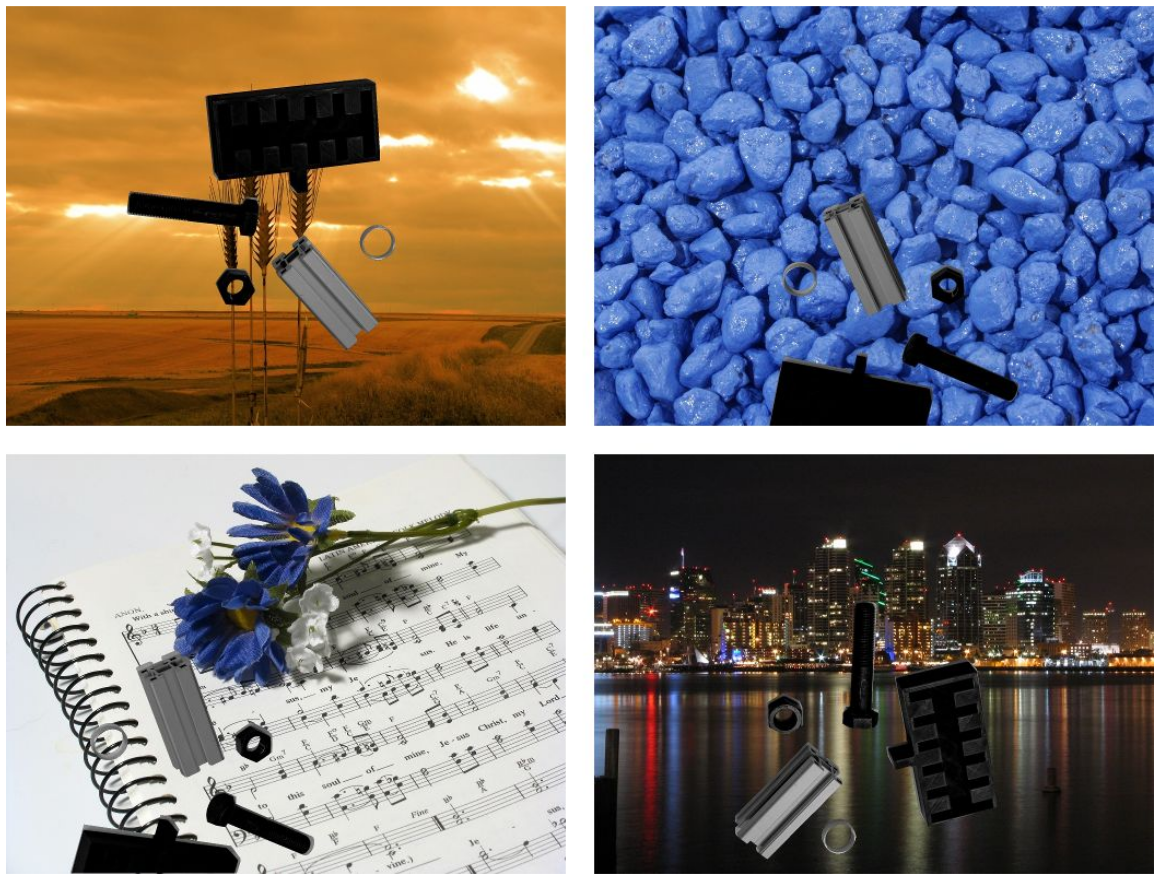
\includegraphics[width=0.8\textwidth]{figures/4_experiments/synthetic_dataset_ex}
    \caption{\textbf{Images from the synthetic RAW Dataset}. In the figure, some examples of the images produced for training the $YOLO_S$ network.}
    \label{fig:synthetic_dataset_ex}
\end{figure}
%\begin{table}
%	\centering
%    \begin{tabular}{| l | l | l |}
%    \hline
%    \textbf{Object Class} & \textbf{$\pmb{YOLO_O}$ - IoU Avg.} & \textbf{$\pmb{YOLO_S}$- IoU Avg.}\\ \hline
%    \emph{Distance\_tube} & \textbf{0.89749} & 0.82526 \\
%    \emph{M20} & \textbf{0.90142} & 0.81673 \\
%    \emph{M20\_100} & \textbf{0.94402} & 0.89050 \\
%    \emph{Cover\_plate\_BOX} & \textbf{0.95479} & 0.92168 \\
%    \emph{S40\_40\_G} & \textbf{0.93904} & 0.82985 \\
%    \hline
%    \end{tabular}
%    \caption{\textbf{YOLO Detection Results}: Both YOLO trained with original RAW Dataset ($YOLO_O$) and with the Synthetic generated dataset ($YOLO_S$).Those results are referred to test images of the original RAW Dataset, not the synthetic generated version.}
%    \label{tab:dl_YOLO_results_unified}
%\end{table}
\subsubsection{Experiment Details}
In the \textbf{Deep Learning} section of \tabref{tab:big_table_results} are reported some results of the test performed with the two networks, namely $YOLO_O$ and $YOLO_S$. The results have been arranged in the same way as the experiment shown before in order to give a comprehensive and consistent way for comparing the two approaches. It is clearly evident that the Deep Learning approaches overcome the shape based ones by more than $\sim10\%$. The main reason why we performed also this other kind of training is that the first network, the $YOLO_O$, seemed to be overfitting the dataset used for training, and the reasons are essentially two:

\begin{itemize}
	\item \textbf{Little size of the training set}: We used only a subset of the overall RAW Dataset, and maybe they are too few images for successfully such a big network (more than 20 convolutional layers + fully connected layers at the end);
	\item \textbf{Too similar images}: images used for the training phase are extremely similar, even if taken from completely different views. Illumination conditions are almost always the same, background is always the same, and so on.
\end{itemize}

We basically claim that such configuration brought the $YOLO_O$ network to overfitting a bit the training set, and clearly evidence of this is given by the result of the detection performed on very different scenes, with objects in a much more cluttered environment. Look at \figref{fig:overfitting_problem} for better understanding the problem. Results show that we overcome a bit the problem of overfitting with the network trained with the standard RAW Dataset.

\begin{figure}
    \centering
    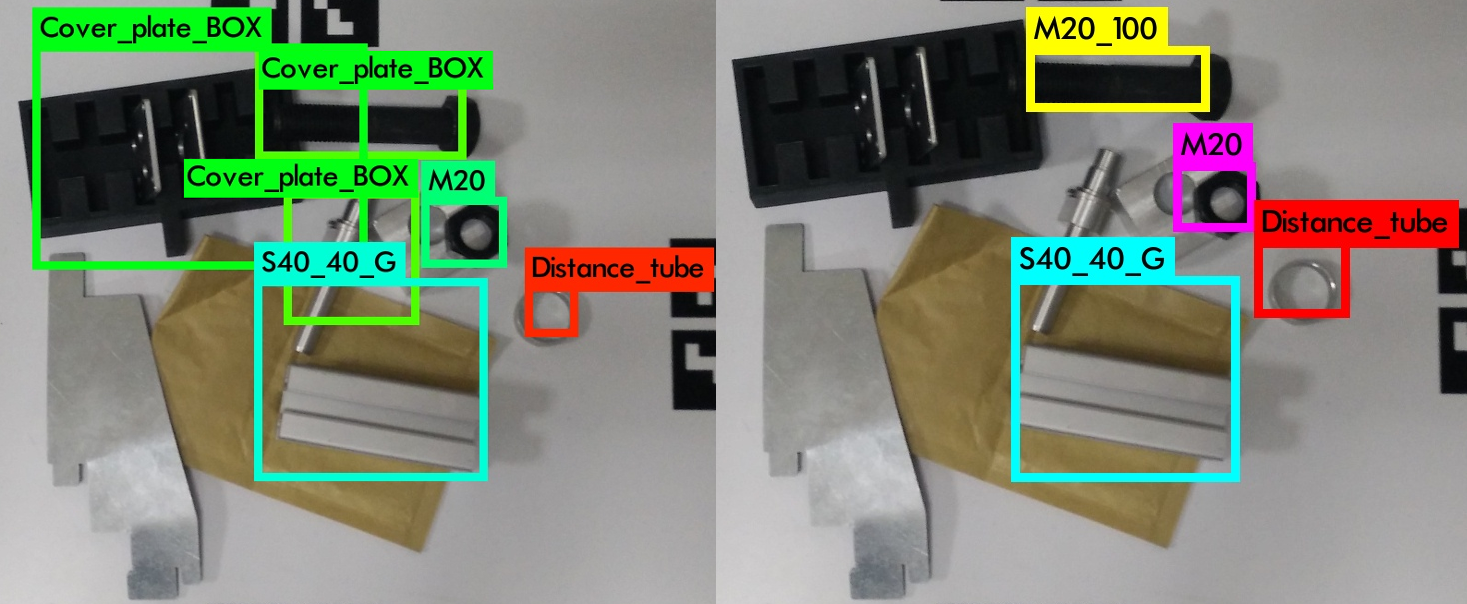
\includegraphics[width=\textwidth]{figures/4_experiments/overfitting_problem}
    \caption{\textbf{Detection Results on totally different scene}. The scene depicted in the image is taken ot of the RAW Dataset, is not part of it essentially. Was built for testing $YOLO_O$ and $YOLO_S$ performances out of the training and test set. On the left there is the result of $YOLO_O$'s detection, on the right the $YOLO_S$'s one. It is clearly evident that $YOLO_S$ is much more robust than the first one. So results show that we overcome a bit the problem of overfitting with the network trained with the standard RAW Dataset.}
    \label{fig:overfitting_problem}
\end{figure}

%\section{Stereo Matching}\label{sec:exp_stereo_matcing}
%To do ...

\section{3D Reconstruction}\label{sec:exp_3d_reconstruction}
To do ...

\section{Discussion}\label{sec:exp_discussion}
To do ...
\newpage
\chapter{Conclusions}\label{ch:conclusions}
To do ...

{
\backmatter
\newpage
\bibliographystyle{splncs}
%\bibliographystyle{apa-good}
\bibliography{references}
}

\newpage
\appendix
\chapter{Appendix}\label{apx:appendix}

\section{FlexSight Project}\label{apx:flexsight}
One of the key challenges in most robotics applications, from robot­aided manufacturing to service robotics applications, is the capability to automatically identify and locate various types of objects, in such a way that the robot can grasp and manipulate them accurately and reliably.

Depending on the application, objects can be regularly disposed in trays, but often they are randomly placed inside bins, or over tables, pallets or conveyor belts. A reliable perception systems is thus required to identify and precisely locate the objects, and to guide robots during the manipulation tasks. Due to the strong impact of these systems in terms of productivity, they have been widely studied in the last decades. Nowadays, many products have been proposed to solve this problem that, under a scientific point of view, it can be considered a very mature topic. Still, almost all the implemented systems assume to deal with rigid, non-deformable objects; moreover, they often assume that object instances of a given object class (e.g., a package)  have all the same size and the same form factor.

FlexSight aims to remove these limiting assumptions, by proposing a perception system that is also able to recognize and localize several types of deformable objects that can be commonly found in many industrial and logistic applications, such as soft sacks, deformable and variable size packaging, food products, articles of clothing, flexible assembly parts, etc ... 
As \emph{deformable objects} (See \figref{fig:deformable_objects_ex}) are intended either as an object that can change its shape or dimensions due to a stress or, with an abuse of notation, as each object that can be obtained from a basic template by applying a resize operator along one or more directions (e.g., a cubic parcel post can be conceptually \emph{deformed} in many kind of parcel posts).

\begin{figure}
    \centering
    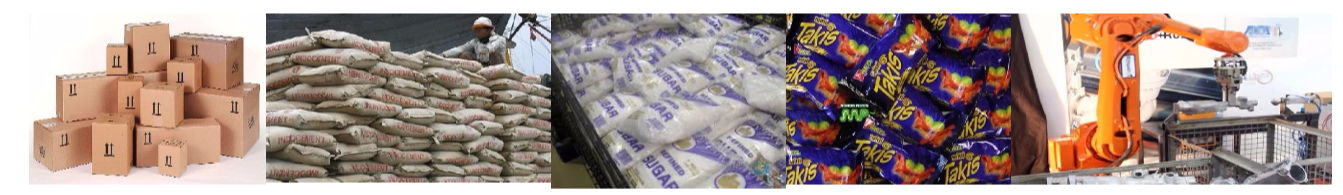
\includegraphics[width=\textwidth]{figures/Appendix/deformable_objects_ex.png}
    \caption{\textbf{Examples of deformable objects}. As deformable objects are intended either as objects that can change their shape or dimensions due to a stress or, with an abuse of notation, as each object that can be obtained from a basic template by applying a resize operator along one or more directions (e.g., a cubic parcel post can be conceptually deformed in many kind of parcel posts).} 
    \label{fig:deformable_objects_ex}
\end{figure}

The main objectives of the FlexSight experiment are:

\begin{itemize}
	\item Enable a robot to perceive a large and widespread class of rigid and deformable objects in an accurate and reliable way, with a particular emphasis on the computational speed of the whole system;
	\item Implement a prototype of a compact industrial sensor (the FlexSight Sensor, FSS for brevity), that integrates inside a robust and small chassis all the required sensors and a processing unit suitable to run the detection and localization algorithms. Our aim is to provide the robot integrators with a sensor that can be easily fitted into conventional robotics cells, thus enabling fully automated and unsupervised procedures in new areas, where usually the intervention of an operator for handling operations is required;
	\item Integrate the FlexSight Sensor inside a working system that will be tested in several industrial and logistic use cases.
\end{itemize}

\subsection{Progress beyond the current state of the technology}\label{subsec:flexsight_related_works}
A wide range of industrial products are packaged in soft bags, sacks or soft packagings. The handling and the palletization of such items during the production is addressed with well engineered and repeatable processes. This is not the case for the industrial end user of these products: they are often randomly placed inside bins or over pallets, so pick\&place operations are performed with forklifts, hoists and/or cranes driven by an operator, leading to significant drawbacks, including health issues (toxic material), hygiene (e.g., in food industry) and efficiency of manual operation. On the other hand, the task of automatically sorting small packages with variable and deformable shapes (e.g., food packages, parcel posts, etc…) inside unstructured environments still remains a challenging problem. A robotic system that can automatically identify, locate, grasp and manipulate all these types of deformable objects is therefore highly desirable.

Many industrial robotics pick\&place systems have been studied and proposed in the last decades. Typically: (1) Either these systems assume to deal with rigid, non deformable objects, where an exact CAD model of the searched objects is provided, or (2) they assume to deal with slightly different instances of the same object class (as in the case of fruits), but objects are placed on a plane or on a conveyor belt and they are isolated, thus making the identification and manipulation relatively easy. Within the FlexSight experiment, we aim to overcome these assumptions. The challenge is first of all technological: even if there is a relevant body of scientific papers dealing with this topic, in most cases they are designed for different purposes (e.g., object categorization) or they are proof of concepts, that is they do not consider the challenges arising in bringing these technologies in highly reliable, industrial environment, that will be addressed below.

Most of the current pick\&place systems employ a recognition and localization system based on vision, 3D depth sensors or RGB-D cameras. They typically employ a standard pipeline of processing blocks:

\begin{figure}[!hbt]
    \centering
    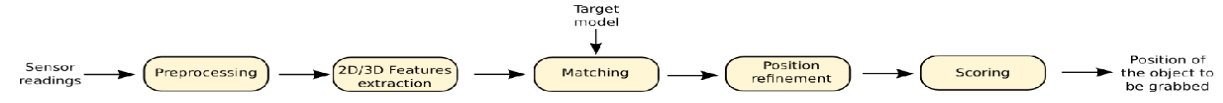
\includegraphics[width=\textwidth]{figures/Appendix/flex_1.png} 
    \label{fig:flex_1}
\end{figure}

Sub-sampling, clustering and noise reduction are often used in the preprocessing blocks, while 2D and/or 3D descriptors are widely used in current systems. The matching block usually aims to associate the extracted features with features pre-computed from a rigid template (e.g., the CAD model) of the object, sample consensus methods are widely used in this case. The result is a set of object candidates, that is refined using iterative optimization strategy (e.g., Iterative Closest Point).

Many research works overcome the assumption of the rigid template model, by proposing several models and techniques to deal with deformable objects but they actually, devoted little effort to develop and test industrial systems able to accurately recognize and localize in 3D, highly deformable and variable objects. In the FlexSight experiment we aim to overcome most of these limitations, enabling an effective \emph{from lab to market} technology transfer: we will investigate among the most promising 3D object modeling solutions, designing an automatic procedure that acquires a multiple-template deformation model (target multi-model) of the objects. The recognition procedure will extract a set of object hypotheses using model-based, visual and 3D structure cues, matched with the target multi-model. Position refinement will be obtained with an efficient optimization procedure that estimates both the position and the deformation parameters of each candidate. Leveraging on the perception outputs, the grasping and manipulation modules will be designed using state of the art hardware and software solutions, enabling reliable and efficient pick\&place operations.

\subsection{FlexSight Project Partners}\label{subsec:flexsight_partners}

\subsubsection{Lab for Cooperative Cognitive Robots (LabRoCoCo, ​coordinating participant​)}
Sapienza Università di Roma is one of the largest and oldest Universities of Italy and Europe.  The Department of Computer, Control and Management Engineering Antonio Ruberti\footnote{https://www.dis.uniroma1.it/} (DIAG) includes about 65 faculty members. Internationally renowned research groups in computer science, system science and management science are active at DIAG. Every year DIAG publishes hundreds of papers in the foremost international journals and conference proceedings.

The research group involved in the project is within the Lab RoCoCo (Cooperative Cognitive Robots)\footnote{http://labrococo.dis.uniroma1.it/} has a strong background in knowledge representation and reasoning, cognitive robotics, information fusion, mapping and localization, object recognition and tracking. multi-robot coordination, robot learning, stereo-vision, vision-based people detection. 
Previous EU-funded projects: SPEAKY for Robots (Echord)\footnote{http://www.echord.info/wikis/website/speaky.html}, RoCKIn\footnote{http://cordis.europa.eu/project/rcn/106855\_en.html}, ROVINA\footnote{http://www.rovina-project.eu/}, Flourish\footnote{http://flourish-project.eu/}.

\subsubsection{IT-Robotics Srl}
Established in 2005, IT+Robotics\footnote{http://www.it-robotics.it/?lang=en} is a spin-off company of the University of Padova. The mission of IT+Robotics is to increase the flexibility of industrial processes by transforming the latest results of the academic research into industrial solutions. IT+Robotics is primarily involved in the fields of robotics and machine vision. IT+Robotics has great experience in random bin picking systems: its product Smart Pick 3D, presented in 2009, is currently used in more than 30 european industrial plants. The products to be collected can vary extensively, and therefore require different hardware and software technologies. By maintaining this approach, over the years IT+Robotics has developed different robot guidance solutions, each of which is designed for a specific product family. IT+Robotics has developed WorkcellSimulator (WCS), a software suite for robot off-line programming, featuring motion planning algorithms based on artificial intelligence methods and vendor independent robot code generation. Moreover, IT+Robotics, in collaboration with Robox, has developed cROS\footnote{http://www.it-robotics.it/products/real-time-systems/cros/?lang=en}, a library written in ANSI C that provides a single thread implementation of the basic features required to implement a ROS (Robot Operating System) node. cROS has been released as open-source in 2015.

\subsubsection{Robox S.p.a.}
Established in 1975, Robox S.p.a.\footnote{http://www.robox.it/it-IT/index.php}, has always been in the forefront of the industrial robotics field. Since the very beginning it has specialized in the design and manufacturing of micro-computerized controllers for robots. From 1987, with the spreading of the Flexible Automation, Robox has exported its know-how to non-robotic applications. Its motion controllers are now employed to control the movement of any machine.

Since 1990 Robox has been included among the Highly Specialized Research Laboratories authorized by the Italian Ministry of Education, University and Research.

Its motion controllers and related tools are applied in a variety of industrial robots, such as: spot welding, arc welding, assembly, plasma cutting, laser cutting, water jet cutting, adhesive coating, pick \& place, palletizing$/$depalletizing, painting, etc. 

%\section{RoboCup@Work}\label{apx:robocupatwork}
%To do ...

%add appendix for dataset class
\end{document}